%% abtex2-modelo-trabalho-academico.tex, v-1.9.5 laurocesar
%% Copyright 2012-2015 by abnTeX2 group at http://www.abntex.net.br/ 
%%
%% This work may be distributed and/or modified under the
%% conditions of the LaTeX Project Public License, either version 1.3
%% of this license or (at your option) any later version.
%% The latest version of this license is in
%%   http://www.latex-project.org/lppl.txt
%% and version 1.3 or later is part of all distributions of LaTeX
%% version 2005/12/01 or later.
%%
%% This work has the LPPL maintenance status `maintained'.
%% 
%% The Current Maintainer of this work is the abnTeX2 team, led
%% by Lauro César Araujo. Further information are available on 
%% http://www.abntex.net.br/
%%
%% This work consists of the files abntex2-modelo-trabalho-academico.tex,
%% abntex2-modelo-include-comandos and abntex2-modelo-references.bib
%%

% ------------------------------------------------------------------------
% ------------------------------------------------------------------------
% abnTeX2: Modelo de Trabalho Academico (tese de doutorado, dissertacao de
% mestrado e trabalhos monograficos em geral) em conformidade com 
% ABNT NBR 14724:2011: Informacao e documentacao - Trabalhos academicos -
% Apresentacao
% ------------------------------------------------------------------------
% ------------------------------------------------------------------------

\documentclass[
	% -- opções da classe memoir --
	12pt,				% tamanho da fonte
	openany,			% capítulos começam em pág ímpar (insere página vazia caso preciso)
	oneside,			% para impressão em verso e anverso. Oposto a oneside
	a4paper,			% tamanho do papel. 
	% -- opções da classe abntex2 --
	%chapter=TITLE,		% títulos de capítulos convertidos em letras maiúsculas
	%section=TITLE,		% títulos de seções convertidos em letras maiúsculas
	%subsection=TITLE,	% títulos de subseções convertidos em letras maiúsculas
	%subsubsection=TITLE,% títulos de subsubseções convertidos em letras maiúsculas
	% -- opções do pacote babel --
	english,			% idioma adicional para hifenização
	brazil				% o último idioma é o principal do documento
	]{abntex2}

% ---
% Pacotes básicos 
% ---
\usepackage{lmodern}			% Usa a fonte Latin Modern			
\usepackage[T1]{fontenc}		% Selecao de codigos de fonte.
\usepackage[utf8]{inputenc}		% Codificacao do documento (conversão automática dos acentos)
\usepackage{lastpage}			% Usado pela Ficha catalográfica
\usepackage{indentfirst}		% Indenta o primeiro parágrafo de cada seção.
\usepackage{color}			% Controle das cores
\usepackage{graphicx}			% Inclusão de gráficos
\usepackage{microtype} 			% para melhorias de justificação
%\usepackage{hyperref}                   % to the figure keep fixed
%\usepackage[justification=centering]{caption} %centrelize all captions
%\captionsetup[figure]{format=hang,indention=-60pt,margin=20pt}
\counterwithin{figure}{section}
\counterwithin{table}{section}


% ---
		
% ---
% Pacotes adicionais, usados apenas no âmbito do Modelo Canônico do abnteX2
% ---
\usepackage{lipsum}				% para geração de dummy text
% ---

% ---
% Pacotes de citações
% ---
\usepackage[brazilian,hyperpageref]{backref}	 % Paginas com as citações na bibl
\usepackage[alf]{abntex2cite}	% Citações padrão ABNT

% --- 
% CONFIGURAÇÕES DE PACOTES
% --- 

% ---
% Configurações do pacote backref
% Usado sem a opção hyperpageref de backref
\renewcommand{\backrefpagesname}{Citado na(s) página(s):~}
% Texto padrão antes do número das páginas
\renewcommand{\backref}{}
% Define os textos da citação
\renewcommand*{\backrefalt}[4]{
	\ifcase #1 %
		Nenhuma citação no texto.%
	\or
		Citado na página #2.%
	\else
		Citado #1 vezes nas páginas #2.%
	\fi}%
% ---

% ---
% Informações de dados para CAPA e FOLHA DE ROSTO
% ---
\titulo{Aplicação de um método estatístico\\ para detecção de \\populações estelares}
\autor{Anna Bárbara de Andrade Queiroz}
\local{Porto Alegre}
\data{2015}
\orientador{Basílio Xavier Santiago}
%\coorientador{}
\instituicao{%
  Universidade Federal do Rio Grande do Sul -- UFRGS
  \par
  Instituto de Física
  \par
  Laboratório Interinstitucional de e-Astronomia}
\tipotrabalho{Trabalho de conclusão de curso}
% O preambulo deve conter o tipo do trabalho, o objetivo, 
% o nome da instituição e a área de concentração 
\preambulo{Trabalho de conclusão de curso apresentado no Instituto              
de Física da Universidade Federal do Rio Grande do Sul, a fim de preencher os 
requisitos para obtenção do título de Bacharel em Física com enfâse em Astrofísica.}
% ---


% ---
% Configurações de aparência do PDF final

% alterando o aspecto da cor azul
%\definecolor{black}%{RGB}{41,5,195}

% informações do PDF
\makeatletter
\hypersetup{
     	%pagebackref=true,
		pdftitle={\@title}, 
		pdfauthor={\@author},
    	pdfsubject={\imprimirpreambulo},
	    pdfcreator={LaTeX with abnTeX2},
		pdfkeywords={abnt}{latex}{abntex}{abntex2}{trabalho acadêmico}, 
		colorlinks=true,       		% false: boxed links; true: colored links
    	linkcolor=black,          	% color of internal links
    	citecolor=black,        		% color of links to bibliography
    	filecolor=magenta,      		% color of file links
		urlcolor=blue,
		bookmarksdepth=4
}
\makeatother
% --- 

% --- 
% Espaçamentos entre linhas e parágrafos 
% --- 

% O tamanho do parágrafo é dado por:
\setlength{\parindent}{1.3cm}

% Controle do espaçamento entre um parágrafo e outro:
\setlength{\parskip}{0.2cm}  % tente também \onelineskip

% ---
% compila o indice
% ---
\makeindex
% ---

% ----
% Início do documento
% ----
\begin{document}

% Seleciona o idioma do documento (conforme pacotes do babel)
%\selectlanguage{english}
\selectlanguage{brazil}

% Retira espaço extra obsoleto entre as frases.
\frenchspacing 

% ----------------------------------------------------------
% ELEMENTOS PRÉ-TEXTUAIS
% ----------------------------------------------------------
% \pretextual

% ---
% Capa
% ---
\imprimircapa
% ---

% ---
% Folha de rosto
% (o * indica que haverá a ficha bibliográfica)
% ---
\imprimirfolhaderosto*
% ---
% Epígrafe
% ---

\begin{epigrafe}
    \vspace*{\fill}
	\begin{flushright}
		\textit{``Astronomy is one of the \\ sublimest fields of human investigation. \\ The mind that grasps its facts \\ and principles receives something \\ of the enlargement and grandeur \\ belonging to the science itself. \\ It is a quickener of devotion'' \\
		(Horace Mann)}
	\end{flushright}
\end{epigrafe}



% ---
% Agradecimentos
% ---
\begin{agradecimentos}
A minha mãe, Neusa, que me ensinou a sempre lutar pelos meus sonhos e nunca desistir deles. \par 

Ao meu orientador Prof. Basílio, por me ensinar a fazer o meu melhor pela profissão que amo. \par

Aos meus irmãos Douglas e Rafael, por todo o carinho, zelo e conforto. \par

Ao meu padrasto José Juan, por ter me ensinado o pensamento científico. \par

Ao meu pai Renato, por me fazer ver as pequenas coisas da vida que realmente valem a pena. \par

A todos os meus colegas/amigos de curso, especialmente a Ivanessa, Felipe, Gustavo, Laís, Thayse e Rafael, que estiveram comigo em ambos os momentos difíceis e divertidos da graduação.  \par

Aos meus colegas de pesquisa, Eduardo, Elmer, Adriano e Marina, por me aconselharem e me ajudarem sempre que necessário. \par

A todos os professores com que tive contato ao longo do curso, por todos os ensinamentos e conselhos. \par

Especialmente agradeço ao Elmer Luque, pela contribuíção de grande parte do trabalho apresentado aqui. 


\end{agradecimentos}
% ---

% ---
% RESUMOS
% ---

% resumo em português
\setlength{\absparsep}{18pt} % ajusta o espaçamento dos parágrafos do resumo
\begin{resumo}

  \qquad O estudo  em detalhe do processo de evolução e formação da Via Láctea cobre diversos aspectos astrofísicos e necessita de observações  fotométricas e espectroscópicas profundas e em grandes volumes Galácticos. Um mecanismo importante proposto para a evolução das galáxias é pela acreção de matéria por atração gravitacional, ou seja, pequenas estruturas estelares entram em órbita ou são completamente fundidas à nossa Galáxia ao longo de sua história. Grandes levantamentos fotométricos, como o Sloan Digital Sky Survey (SDSS) e o Dark Energy Survey (DES), vêm nos dando a oportunidade de detectar e fazer um censo dessas estruturas estelares que ainda se encontram nos limites da Via Láctea, o halo Galáctico. \par
  \qquad Inspirados por essas questões e pelos recentes levantamentos fotométricos, desenvolvemos o algoritimo SparSEx, um método para detecção de novas subestruturas estelares. O método é uma combinação da técnica de matched filter com um simulador de populações estelares simples e um detector sistemático de sobredensidades. O método foi validado pela busca de subestruturas já conhecidas, tais como aglomerados estelares, galáxias anãs e correntes estelares,  em regiões cobertas  pelo Baryon Oscillation Spectroscopy Survey (BOSS) e pelo SDSS. Nós recuperamos com sucesso todos os aglomerados e anãs conhecidas com alta significância, além de também recuperarmos a cauda de maré da galáxia anã de Sagitário. \par
  \qquad Após a validação do método, aplicamos o algoritmo aos dados  dos dois primeiros anos do DES, materializados pelos catálogos de uso interno chamados respectivamente de Y1A1 e Y2Q1. Essa aplicação nos revelou 17 candidatos a galáxias anãs nunca antes detectados. Muitas dessas  subestruturas  estão próximas do sistema de Magalhães e têm baixa luminosidade. Esses resultados, obtidos em conjunto com colaboração do DES, foram publicados em fevereiro e agosto deste ano. \par
  \qquad  Esperamos que o algoritimo SparSEx possa ser usado em dados futuros do DES e também em novos levantamentos fotométricos, como, por exemplo, o Large Synoptic Survey Telescope, aumentando nosso conhecimento e acurácia sobre as subestruturas existentes no halo Galáctico e, por conseguinte, nosso conhecimento sobre a evolução da Via Láctea. 
	
 \textbf{Palavras-chave}: Via Láctea. Subestruturas. Halo Galáctico.
\end{resumo}

% resumo em inglês
\begin{resumo}[Abstract]
 \begin{otherlanguage*}{english}

\qquad The detailed study of the Milk Way  process of formation and evolution covers a wide range of astrophysical aspects and needs deep photometric and spectroscopic observations on large Galactic volumes. A suggested important mechanism for the evolution of galaxies is through  the matter accretion due to gravitational attraction. In other words, small stellar structures  come into orbiting or are completely consumed by our Galaxy on the course of its history.  Wide photometric surveys, such as Sloan Digital Survey (SDSS)  and  the  Dark Energy Survey (DES), give us the new opportunity to detect and complete the census of these stellar structures that are still in the limits of the Milk Way, in the Galactic halo. \par 
\qquad Inspired by these questions and by the recent photometric surveys, we developed the SparSEx algorithm, a method for detecting new stellar substructures. The method is a combination of the matched filter technique with a simulator of simple stellar population and a systematic detector of over-densities. The method was validated by the search for knew substructures, as globular clusters,  dwarf galaxies and stellar streams,  on regions covered by the Baryon Oscillation Spectroscopy Survey (BOSS) and by SDSS. We successfully recover all the knew globular clusters and dwarf galaxies with high significance. We also recovered  the Sagittarius dwarf stellar stream. \par
\qquad After the method validation, we applied the algorithm to the data of the two first years of DES, which are contained in the internal collaboration called  respectively by Y1A1 and Y2Q1. This application revealed 17 dwarf galaxy candidates never detected before. Many of these substructure are near the Magellanic clouds, and are poor stellar populations. These results, which were obtained by our method and also by other methods inside the DES collaboration, were published in  February and August of this year. \par
\qquad We hope that the SparSEx algorithm can be used on future data from DES and also new photometric surveys,  like, for example, the  Large Synoptic Survey Telescope. This will  increase our knowledge and accuracy about the existing substructures that are located in the Galactic halo, and therefore our knowledge about the Milk way evolution.
   \vspace{\onelineskip}
 
   \noindent 
   \textbf{Keywords}: Milk Way. Substructures. Galactic Halo.
 \end{otherlanguage*}
\end{resumo}

% ---

% ---
% inserir lista de abreviaturas e siglas
% ---
\begin{siglas}
  \item[VL] Via Láctea
  \item[DES] Dark Energy Survey
  \item[Y1A1] Catálogo referente aos dados do primeiro ano do Dark Energy Survey
  \item[Y2Q1] Catálogo referente aos dados do segundo ano do Dark Energy Survey
  \item[SDSS] Sloan Digital Sky Survey
  \item[BOSS] Baryon Oscillation Spectroscopy Survey 
  \item[2MASS] Two Micron All Sky Survey
  \item[MF] Matched Filter
  \item[CMD] Diagrama Cor Magnitude
  \item[SSP] Populações Estelares Simples
  \item[PDF] Função distribuição de probabilidade
  \item[IMF] Função de massa inicial
  \item[CTIO] Cerro Tololo Inter-American Observatory
  \item[DESDM] Dark Energy Survey Data Management

\end{siglas}
% ---


% ---
% inserir o sumario
% ---
\pdfbookmark[0]{\contentsname}{toc}
\tableofcontents*
\cleardoublepage
% ---



% ----------------------------------------------------------
% ELEMENTOS TEXTUAIS
% ----------------------------------------------------------
\textual

% ----------------------------------------------------------
% Introdução (exemplo de capítulo sem numeração, mas presente no Sumário)
% ----------------------------------------------------------
\chapter*[Introdução]{Introdução}
\addcontentsline{toc}{chapter}{Introdução}
% ----------------------------------------------------------

\qquad Chamamos de  satélites da Via Láctea (VL) galáxias anãs e aglomerados globulares que se encontram nos limites do halo Galáctico e estão gravitacionalmente ligados a VL. Estes sistemas são em geral velhos, pobres em metal e as galáxias anãs também são ricas em matéria escura. Por essas características, esses satélites carregam ricas informações sobre a formação e evolução da nossa Galáxia. Dentre as muitas aplicações para a detecção dos satélites estão: o modelamento do componente esferoidal da Galáxia, descrição dos episódios iniciais de acreção de massa e até mesmo a natureza das partículas de matéria escura. Muitas das recentes descobertas de satélites incluem estruturas com raios, massas, luminosidades e brilho superficial bem pequenos em comparação a outras galáxias ou mesmo a aglomerados globulares, o que também nos permite estender as relações de escala para esses parâmetros. \par
\qquad Antes do advento de grandes surveys como o Sloan Digital Sky Survey (SDSS)\footnote{\url{http://www.sdss.org/}}, o Two Micron All Sky Survey (2MASS)\footnote{\url{http://www.ipac.caltech.edu/2mass/}} e o Dark Energy Survey (DES)\footnote{\url{http://www.darkenergysurvey.org/}},  conhecíamos somente alguns satélites, cerca de 12 galáxias anãs \cite{2012AJ....144....4M} incluindo a pequena e grande nuvem de Magalhães, que podem ser avistadas a olho nu, e cerca de 50 aglomerados globulares situados nas regiões externas do halo Galáctico \cite{1996AJ....112.1487H}. O censo dessas subestruturas mudou drasticamente nos últimos quinze anos devido a esses grandes levantamentos \cite{2005astro.ph..6460W,2006AAS...20917805Z,2010ApJ...712L.103B,2007MNRAS.382..515V} . Já podemos contabilizar, Levando em conta as mais novas descobertas do DES, cerca de 36 galáxias anãs e 57 aglomerados globulares. Diversos outros aglomerados estelares foram descobertos durante os últimos anos, porém a sua classificação como galáxia anã ou aglomerado globular ainda não é clara \cite{2010ApJ...712L.103B,2013ApJ...767..101B,2005AJ....129.2692W,2015ApJ...804L..44K,2015ApJ...803...63K}.  Algumas características que distinguem  galáxias anãs de aglomerados globulares são:  a dispersão de metalicidades indicando múltiplas gerações de formação estelar, potencial gravitacional profundo o suficiente para reter ejeções de supernova, seu local no espaço de luminosidade X raio físico e também ser um sistema rico em matéria escura \cite{2012AJ....144...76W}. \par
Foi no último ano que 17 candidatos a galáxias anãs foram detectadas através do DES \cite{2015ApJ...807...50B,2015arXiv150803622T}. Desses 17 candidatos, 5 estão em local ambíguo  no espaço luminosidade X raio físico para distinção entre galáxia anã e aglomerado globular. Até o momento 3 dos 17 candidatos foram confirmados como galáxias anãs  através de observações espectroscópicas que mostram suas assinaturas cinemáticas e químicas são consistentes com os de uma galáxia \cite{2015ApJ...811...62K,2015ApJ...810...56K}.  

Na Figura \ref{fig:dwarfcenso} \footnote{A Figura \ref{fig:dwarfcenso} foi retirada de \cite{2015ApJ...807...50B,2015arXiv150803622T}}  vemos um  mapa Galáctico com a distribuição espacial de todas as galáxias anãs conhecidas até o momento, inclusive os novos candidatos detectados com os dados dos dois primeiros anos do DES, chamamos de  Y1A1 os dados referentes ao primeiro ano e Y2Q1 os dados referentes ao segundo ano. O DES  ainda está coletando dados observacionais com a Dark Energy Camera (DECam) acoplada ao Blanco 4-meter Telescope que se  situa no sítio observacional de Cerro Tololo. Portanto espera-se que o DES revele ainda mais alguns satélites da VL. Em fato \cite{2008ApJ...688..277T} previu que seriam descobertos de 19 a 37 objetos no DES, assumindo que as características de detecção desse levantamento são parecidas com as do SDSS.

\begin{figure}[h]
\begin{center}
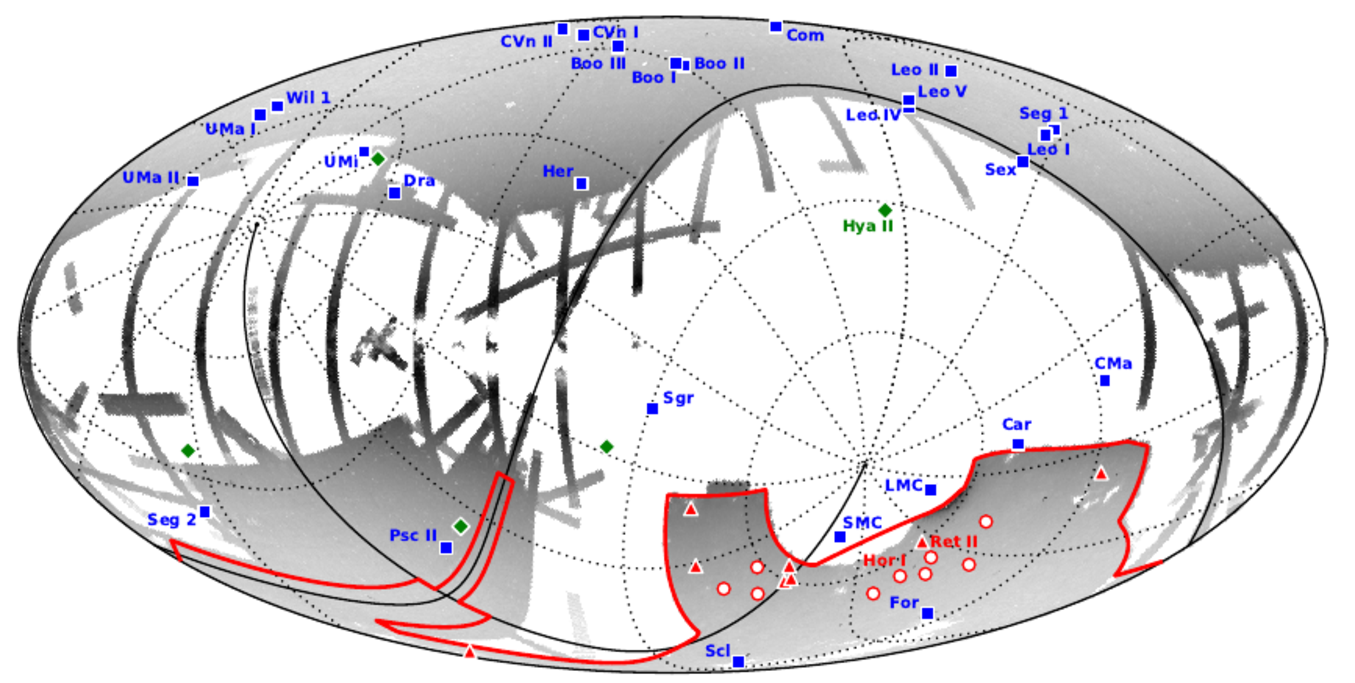
\includegraphics[width=12cm]{figuras/censodg.pdf}
\caption{\textit{Mapa com a distribuição dos satélites da VL. O footprint do DES está representado pelo delineamento vermelho, os triângulos vermelhos \cite{2012AJ....144...76W} representam os 8 candidatos à galáxias anãs detectados com os dados do Y1A1, os círculos vermelhos \cite{2015ApJ...807...50B,2015arXiv150803622T} representam os 9 candidatos detectados com os dados do Y2Q1, outras cinco recentes descobertas fora do footprint do DES estão marcadas por losangos verdes \cite{2015ApJ...802L..18L,2015ApJ...804L...5M, 2015ApJ...804L..44K,2015ApJ...813...44L} e os quadrados azuis \cite{2012AJ....144....4M} representam galáxias já detectadas antes de 2015. A figura está em coordenadas Galácticas, com a grade pontilhada mostrando a projeção das coordenadas equatoriais. O mapa mostra a densidade logarítmica de estrelas em escala de cores cinza.}}
\label{fig:dwarfcenso}
\end{center}
\end{figure}
\vspace{0.5cm}

Alguns dos satélites da VL estão sofrendo perda de massa:  devido a processos dinâmicos e gravitacionais de interação com a Via Láctea (VL), as estrelas são jogadas para fora de suas galáxias, formando correntes estelares no interior da VL \cite{1991ApJ...379...52W}. Fazendo-se um modelamento de correntes estelares é possível determinar potencial gravitacional da Galáxia \cite{2014ApJ...795...94B} . Para um modelamento não tendencioso é importante termos os dados de várias correntes estelares. É bastante provável que alguns dos progenitores já tenham sidos totalmente consumidos pela VL, completando o processo de acreção de massa pela Galáxia. A corrente estelar de Virgo é um desses exemplos, detectada através de observações espectroscópicas de estrelas RR Lyraes \cite{2006RMxAC..26...70D}, acredita-se que esta corrente pertenceu a  uma galáxia anã esferoidal satélite da VL que já foi completamente consumida \cite{2012ApJ...753..145C}. Outro exemplo é a corrente estelar de Sagitário, galáxia esferoidal que está em processo de ruptura \cite{2001ApJ...547L.133I}. A corrente de Sagitário se estende  em  uma órbita polar dando uma volta completa em torno da Galáxia. \par

O surto dessas descobertas também é acompanhado pela descoberda de sistemas com bem baixa luminosidade ($-3.0 \le Mv \le 0$) e pequenos raios a meia luz ($\le$ 10pc), sendo mais consistentes com aglomerados globulares \cite{2007ApJ...669..337K,2010ApJ...712L.103B, 2011AJ....142...88F,2013ApJ...767..101B}.  Muitos dos aglomerados do halo Galáctico, podem ter sido formados em galáxias anãs que estão em órbita ou foram acretadas pela VL. Isto é reforçado pelo fato de que vários aglomerados são encontrados perto da corrente estelar de Sagitário e do sistema magalânico \cite{2010ApJ...718.1128L,2015MNRAS.453.3568D}.  Porém essas recentes descobertas, que varrem luminosidades muito baixas, deixam a distinção entre aglomerados globulares e galáxias anãs cada vez menos clara. Por esse motivo é importante persistir em um censo completo dos satélites mais tênues da Galáxia e caracterizá-los em termos de estrutura, população estelar e quantidade de matéria escura. Extrapolações dos resultados do SDSS, sobre a função de luminosidade dos satélites indicam que esse censo ainda está bem incompleto \cite{2008ApJ...688..277T, 2014ApJ...795L..13H}. \par 

Descrevemos nesse trabalho um método para detecção de populações estelares resolvidas, como galáxias anãs, corretes estelares e aglomerados globulares. O método consiste da aplicação da técnica de matched filter (MF). O MF faz uma comparação estatística entre uma dada população de estrelas e a amostra observacional,  realçando as estrelas que são mais compatíveis com a população. O cálculo estatístico é feito em um espaço binado de posição e Diagrama Cor Magnitude (CMD). Esta técnica de MF é uma extensão do código Sparse, construído para a detecção da corrente estelar do aglomerado globular NGC 2298, \cite{2011MNRAS.416..393B}.
A maioria dos autores tem usado a técnica do MF para detectar estrelas pertencentes a uma população estelar previamente conhecida, \cite{2012ASPC..458..219G,2009AAS...21344217D}. Para procurar por uma estrutura não conhecida precisamos de uma grade de diferentes populações estelares, variando em um intervalo largo de idades, metalicidades e distâncias. Para essa tarefa usamos um simulador de populações estelares simples (SSP), o GenCMD, que utiliza modelos de evolução estelar de Padova \cite{2012MNRAS.427..127B} para simular as diferentes idades e metalicidades. \par

A aplicação do MF não nos dá as coordenadas dos candidatos a subestrutura diretamente, ele só gera um mapa onde tais candidatos podem ser localizados posteriormente. Para então encontrarmos as coordenadas dos candidatos, podemos fazer uma inspeção visual  ou usarmos um código de busca sistemática por sobredensidades. Como aplicamos o MF para uma grande quantidade de modelos de SSP,  a primeira opção se torna muito demorada devido ao grande tempo gasto na inspeção visual. Decidimos então aplicar o código de busca por sobredensidade Sextractor  \cite{1996A&AS..117..393B}.
	Chamamos o algorítimo de detecção de subestruturas de SparSEx, sendo este portanto a combinação dos códigos Sparse e Sextractor. Descrevemos também  a validação deste método por meio da recuperação de subestruturas já conhecidas. Tanto galáxias anãs, aglomerados globulares e correntes estelares foram recuperados com sucesso nos dados do SDSS. Por fim o método foi aplicado nos dados do DES, Y1A1 e Y2Q1,  onde combinado com outros dois métodos de busca de  dentro da colaboração,  foram encontradas os 16 satélites da VL e o aglomerado estelar DES-1 \cite{2015ApJ...807...50B,2015arXiv150803622T,2015arXiv150802381L}.   


% ----------------------------------------------------------
% PARTE
% ----------------------------------------------------------
%\part{Preparação}
%\chapter{Objetivos}
\chapter*[Objetivos]{Objetivos}
\addcontentsline{toc}{chapter}{Objetivos}

%\section{algo}
% ----------------------------------------------------------
%%% abtex2-modelo-include-comandos.tex, v<VERSION> laurocesar
%% Copyright 2012-2015 by abnTeX2 group at http://www.abntex.net.br/ 
%%
%% This work may be distributed and/or modified under the
%% conditions of the LaTeX Project Public License, either version 1.3
%% of this license or (at your option) any later version.
%% The latest version of this license is in
%%   http://www.latex-project.org/lppl.txt
%% and version 1.3 or later is part of all distributions of LaTeX
%% version 2005/12/01 or later.
%%
%% This work has the LPPL maintenance status `maintained'.
%% 
%% The Current Maintainer of this work is the abnTeX2 team, led
%% by Lauro César Araujo. Further information are available on 
%% http://www.abntex.net.br/
%%
%% This work consists of the files abntex2-modelo-include-comandos.tex
%% and abntex2-modelo-img-marca.pdf
%%

% ---
% Este capítulo, utilizado por diferentes exemplos do abnTeX2, ilustra o uso de
% comandos do abnTeX2 e de LaTeX.
% ---
 
\chapter{Resultados de comandos}\label{cap_exemplos}

\chapterprecis{Isto é uma sinopse de capítulo. A ABNT não traz nenhuma
normatização a respeito desse tipo de resumo, que é mais comum em romances 
e livros técnicos.}\index{sinopse de capítulo}

% ---
\section{Codificação dos arquivos: UTF8}
% ---

A codificação de todos os arquivos do \abnTeX\ é \texttt{UTF8}. É necessário que
você utilize a mesma codificação nos documentos que escrever, inclusive nos
arquivos de base bibliográficas |.bib|.

% ---
\section{Citações diretas}
\label{sec-citacao}
% ---

\index{citações!diretas}Utilize o ambiente \texttt{citacao} para incluir
citações diretas com mais de três linhas:

\begin{citacao}
As citações diretas, no texto, com mais de três linhas, devem ser
destacadas com recuo de 4 cm da margem esquerda, com letra menor que a do texto
utilizado e sem as aspas. No caso de documentos datilografados, deve-se
observar apenas o recuo \cite[5.3]{NBR10520:2002}.
\end{citacao}

Use o ambiente assim:

\begin{verbatim}
\begin{citacao}
As citações diretas, no texto, com mais de três linhas [...] deve-se observar
apenas o recuo \cite[5.3]{NBR10520:2002}.
\end{citacao}
\end{verbatim}

O ambiente \texttt{citacao} pode receber como parâmetro opcional um nome de
idioma previamente carregado nas opções da classe (\autoref{sec-hifenizacao}). Nesse
caso, o texto da citação é automaticamente escrito em itálico e a hifenização é
ajustada para o idioma selecionado na opção do ambiente. Por exemplo:

\begin{verbatim}
\begin{citacao}[english]
Text in English language in italic with correct hyphenation.
\end{citacao}
\end{verbatim}

Tem como resultado:

\begin{citacao}[english]
Text in English language in italic with correct hyphenation.
\end{citacao}

\index{citações!simples}Citações simples, com até três linhas, devem ser
incluídas com aspas. Observe que em \LaTeX as aspas iniciais são diferentes das
finais: ``Amor é fogo que arde sem se ver''.

% ---
\section{Notas de rodapé}
% ---

As notas de rodapé são detalhadas pela NBR 14724:2011 na seção 5.2.1\footnote{As
notas devem ser digitadas ou datilografadas dentro das margens, ficando
separadas do texto por um espaço simples de entre as linhas e por filete de 5
cm, a partir da margem esquerda. Devem ser alinhadas, a partir da segunda linha
da mesma nota, abaixo da primeira letra da primeira palavra, de forma a destacar
o expoente, sem espaço entre elas e com fonte menor
\citeonline[5.2.1]{NBR14724:2011}.}\footnote{Caso uma série de notas sejam
criadas sequencialmente, o \abnTeX\ instrui o \LaTeX\ para que uma vírgula seja
colocada após cada número do expoente que indica a nota de rodapé no corpo do
texto.}\footnote{Verifique se os números do expoente possuem uma vírgula para
dividi-los no corpo do texto.}. 


% ---
\section{Tabelas}
% ---

\index{tabelas}A \autoref{tab-nivinv} é um exemplo de tabela construída em
\LaTeX.

\begin{table}[htb]
\ABNTEXfontereduzida
\caption[Níveis de investigação]{Níveis de investigação.}
\label{tab-nivinv}
\begin{tabular}{p{2.6cm}|p{6.0cm}|p{2.25cm}|p{3.40cm}}
  %\hline
   \textbf{Nível de Investigação} & \textbf{Insumos}  & \textbf{Sistemas de Investigação}  & \textbf{Produtos}  \\
    \hline
    Meta-nível & Filosofia\index{filosofia} da Ciência  & Epistemologia &
    Paradigma  \\
    \hline
    Nível do objeto & Paradigmas do metanível e evidências do nível inferior &
    Ciência  & Teorias e modelos \\
    \hline
    Nível inferior & Modelos e métodos do nível do objeto e problemas do nível inferior & Prática & Solução de problemas  \\
   % \hline
\end{tabular}
\legend{Fonte: \citeonline{van86}}
\end{table}

Já a \autoref{tabela-ibge} apresenta uma tabela criada conforme o padrão do
\citeonline{ibge1993} requerido pelas normas da ABNT para documentos técnicos e
acadêmicos.

\begin{table}[htb]
\IBGEtab{%
  \caption{Um Exemplo de tabela alinhada que pode ser longa
  ou curta, conforme padrão IBGE.}%
  \label{tabela-ibge}
}{%
  \begin{tabular}{ccc}
  \toprule
   Nome & Nascimento & Documento \\
  \midrule \midrule
   Maria da Silva & 11/11/1111 & 111.111.111-11 \\
  \midrule 
   João Souza & 11/11/2111 & 211.111.111-11 \\
  \midrule 
   Laura Vicuña & 05/04/1891 & 3111.111.111-11 \\
  \bottomrule
\end{tabular}%
}{%
  \fonte{Produzido pelos autores.}%
  \nota{Esta é uma nota, que diz que os dados são baseados na
  regressão linear.}%
  \nota[Anotações]{Uma anotação adicional, que pode ser seguida de várias
  outras.}%
  }
\end{table}


% ---
\section{Figuras}
% ---

\index{figuras}Figuras podem ser criadas diretamente em \LaTeX,
como o exemplo da \autoref{fig_circulo}.

\begin{figure}[htb]
	\caption{\label{fig_circulo}A delimitação do espaço}
	\begin{center}
	    \setlength{\unitlength}{5cm}
		\begin{picture}(1,1)
		\put(0,0){\line(0,1){1}}
		\put(0,0){\line(1,0){1}}
		\put(0,0){\line(1,1){1}}
		\put(0,0){\line(1,2){.5}}
		\put(0,0){\line(1,3){.3333}}
		\put(0,0){\line(1,4){.25}}
		\put(0,0){\line(1,5){.2}}
		\put(0,0){\line(1,6){.1667}}
		\put(0,0){\line(2,1){1}}
		\put(0,0){\line(2,3){.6667}}
		\put(0,0){\line(2,5){.4}}
		\put(0,0){\line(3,1){1}}
		\put(0,0){\line(3,2){1}}
		\put(0,0){\line(3,4){.75}}
		\put(0,0){\line(3,5){.6}}
		\put(0,0){\line(4,1){1}}
		\put(0,0){\line(4,3){1}}
		\put(0,0){\line(4,5){.8}}
		\put(0,0){\line(5,1){1}}
		\put(0,0){\line(5,2){1}}
		\put(0,0){\line(5,3){1}}
		\put(0,0){\line(5,4){1}}
		\put(0,0){\line(5,6){.8333}}
		\put(0,0){\line(6,1){1}}
		\put(0,0){\line(6,5){1}}
		\end{picture}
	\end{center}
	\legend{Fonte: os autores}
\end{figure}

Ou então figuras podem ser incorporadas de arquivos externos, como é o caso da
\autoref{fig_grafico}. Se a figura que ser incluída se tratar de um diagrama, um
gráfico ou uma ilustração que você mesmo produza, priorize o uso de imagens
vetoriais no formato PDF. Com isso, o tamanho do arquivo final do trabalho será
menor, e as imagens terão uma apresentação melhor, principalmente quando
impressas, uma vez que imagens vetorias são perfeitamente escaláveis para
qualquer dimensão. Nesse caso, se for utilizar o Microsoft Excel para produzir
gráficos, ou o Microsoft Word para produzir ilustrações, exporte-os como PDF e
os incorpore ao documento conforme o exemplo abaixo. No entanto, para manter a
coerência no uso de software livre (já que você está usando \LaTeX e \abnTeX),
teste a ferramenta \textsf{InkScape}\index{InkScape}
(\url{http://inkscape.org/}). Ela é uma excelente opção de código-livre para
produzir ilustrações vetoriais, similar ao CorelDraw\index{CorelDraw} ou ao Adobe
Illustrator\index{Adobe Illustrator}. De todo modo, caso não seja possível
utilizar arquivos de imagens como PDF, utilize qualquer outro formato, como
JPEG, GIF, BMP, etc. Nesse caso, você pode tentar aprimorar as imagens
incorporadas com o software livre \textsf{Gimp}\index{Gimp}
(\url{http://www.gimp.org/}). Ele é uma alternativa livre ao Adobe
Photoshop\index{Adobe Photoshop}.

\begin{figure}[htb]
	\caption{\label{fig_grafico}Gráfico produzido em Excel e salvo como PDF}
	\begin{center}
	    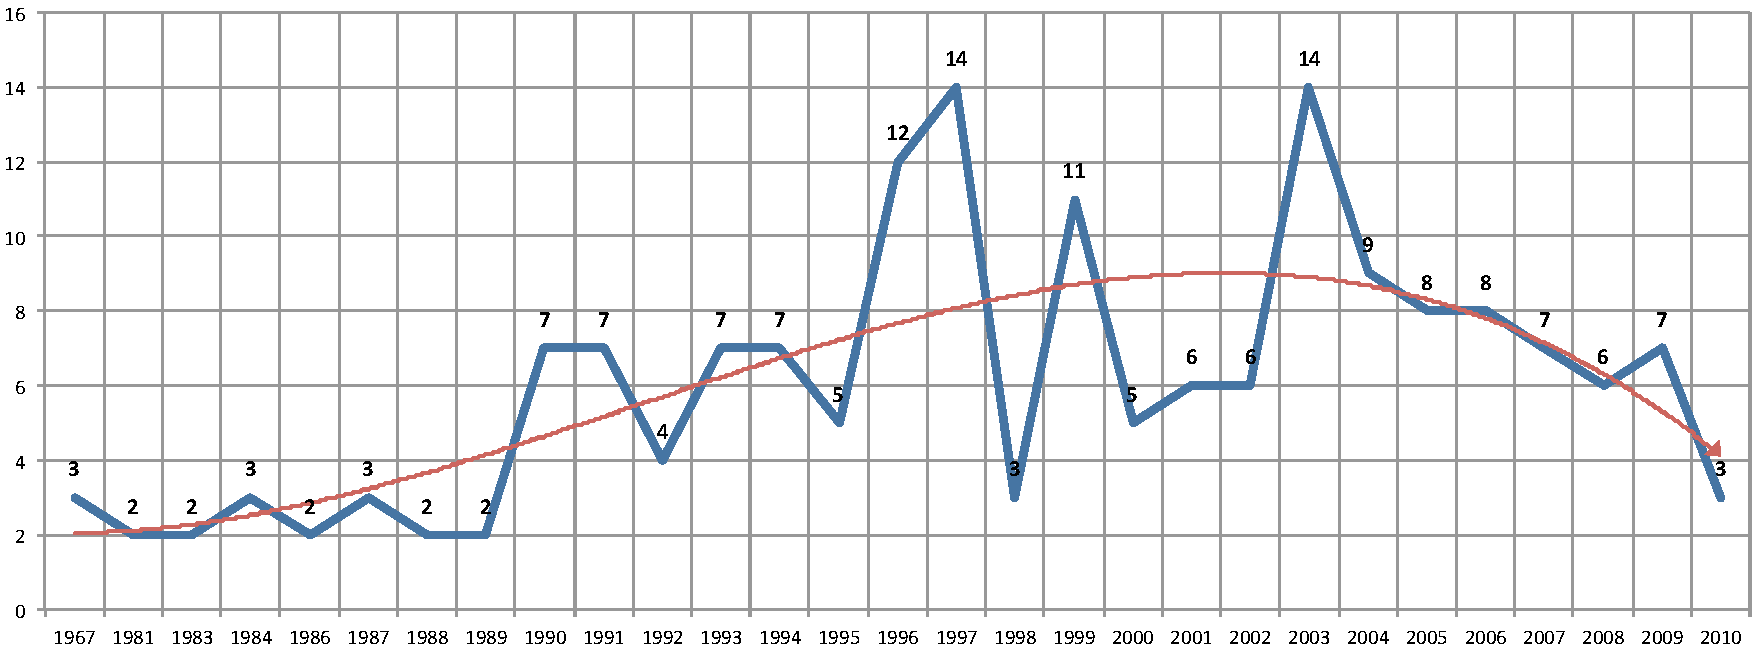
\includegraphics[scale=0.5]{abntex2-modelo-img-grafico.pdf}
	\end{center}
	\legend{Fonte: \citeonline[p. 24]{araujo2012}}
\end{figure}

% ---
\subsection{Figuras em \emph{minipages}}
% ---

\emph{Minipages} são usadas para inserir textos ou outros elementos em quadros
com tamanhos e posições controladas. Veja o exemplo da
\autoref{fig_minipage_imagem1} e da \autoref{fig_minipage_grafico2}.

\begin{figure}[htb]
 \label{teste}
 \centering
  \begin{minipage}{0.4\textwidth}
    \centering
    \caption{Imagem 1 da minipage} \label{fig_minipage_imagem1}
    
\includegraphics[scale=0.9]{abntex2-modelo-img-marca.pdf}
    \legend{Fonte: Produzido pelos autores}
  \end{minipage}
  \hfill
  \begin{minipage}{0.4\textwidth}
    \centering
    \caption{Grafico 2 da minipage} \label{fig_minipage_grafico2}
    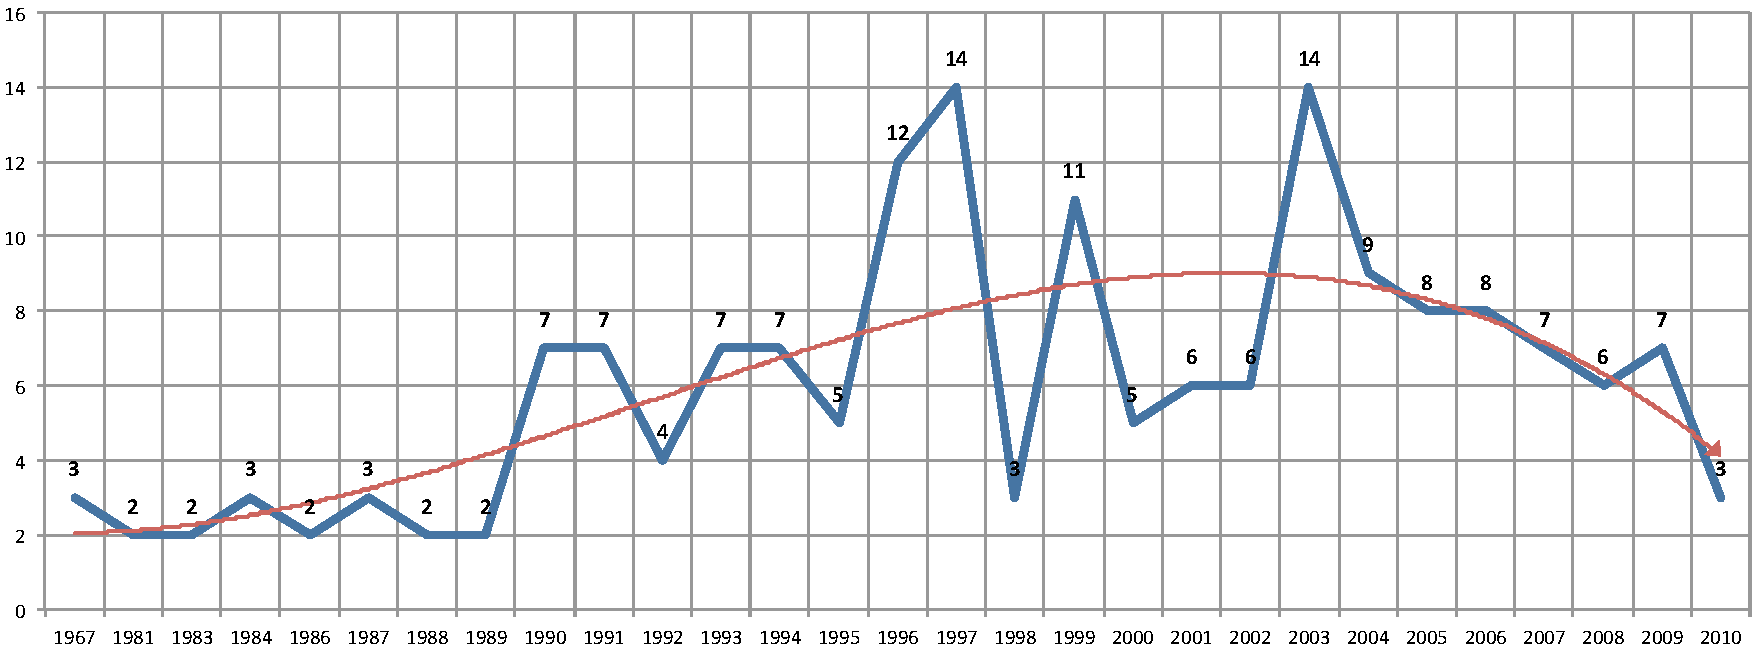
\includegraphics[scale=0.2]{abntex2-modelo-img-grafico.pdf}
    \legend{Fonte: \citeonline[p. 24]{araujo2012}}
  \end{minipage}
\end{figure}

Observe que, segundo a \citeonline[seções 4.2.1.10 e 5.8]{NBR14724:2011}, as
ilustrações devem sempre ter numeração contínua e única em todo o documento:

\begin{citacao}
Qualquer que seja o tipo de ilustração, sua identificação aparece na parte
superior, precedida da palavra designativa (desenho, esquema, fluxograma,
fotografia, gráfico, mapa, organograma, planta, quadro, retrato, figura,
imagem, entre outros), seguida de seu número de ordem de ocorrência no texto,
em algarismos arábicos, travessão e do respectivo título. Após a ilustração, na
parte inferior, indicar a fonte consultada (elemento obrigatório, mesmo que
seja produção do próprio autor), legenda, notas e outras informações
necessárias à sua compreensão (se houver). A ilustração deve ser citada no
texto e inserida o mais próximo possível do trecho a que se
refere. \cite[seções 5.8]{NBR14724:2011}
\end{citacao}

% ---
\section{Expressões matemáticas}
% ---

\index{expressões matemáticas}Use o ambiente \texttt{equation} para escrever
expressões matemáticas numeradas:

\begin{equation}
  \forall x \in X, \quad \exists \: y \leq \epsilon
\end{equation}

Escreva expressões matemáticas entre \$ e \$, como em $ \lim_{x \to \infty}
\exp(-x) = 0 $, para que fiquem na mesma linha.

Também é possível usar colchetes para indicar o início de uma expressão
matemática que não é numerada.

\[
\left|\sum_{i=1}^n a_ib_i\right|
\le
\left(\sum_{i=1}^n a_i^2\right)^{1/2}
\left(\sum_{i=1}^n b_i^2\right)^{1/2}
\]

Consulte mais informações sobre expressões matemáticas em
\url{https://github.com/abntex/abntex2/wiki/Referencias}.

% ---
\section{Enumerações: alíneas e subalíneas}
% ---

\index{alíneas}\index{subalíneas}\index{incisos}Quando for necessário enumerar
os diversos assuntos de uma seção que não possua título, esta deve ser
subdividida em alíneas \cite[4.2]{NBR6024:2012}:

\begin{alineas}

  \item os diversos assuntos que não possuam título próprio, dentro de uma mesma
  seção, devem ser subdivididos em alíneas; 
  
  \item o texto que antecede as alíneas termina em dois pontos;
  \item as alíneas devem ser indicadas alfabeticamente, em letra minúscula,
  seguida de parêntese. Utilizam-se letras dobradas, quando esgotadas as
  letras do alfabeto;

  \item as letras indicativas das alíneas devem apresentar recuo em relação à
  margem esquerda;

  \item o texto da alínea deve começar por letra minúscula e terminar em
  ponto-e-vírgula, exceto a última alínea que termina em ponto final;

  \item o texto da alínea deve terminar em dois pontos, se houver subalínea;

  \item a segunda e as seguintes linhas do texto da alínea começa sob a
  primeira letra do texto da própria alínea;
  
  \item subalíneas \cite[4.3]{NBR6024:2012} devem ser conforme as alíneas a
  seguir:

  \begin{alineas}
     \item as subalíneas devem começar por travessão seguido de espaço;

     \item as subalíneas devem apresentar recuo em relação à alínea;

     \item o texto da subalínea deve começar por letra minúscula e terminar em
     ponto-e-vírgula. A última subalínea deve terminar em ponto final, se não
     houver alínea subsequente;

     \item a segunda e as seguintes linhas do texto da subalínea começam sob a
     primeira letra do texto da própria subalínea.
  \end{alineas}
  
  \item no \abnTeX\ estão disponíveis os ambientes \texttt{incisos} e
  \texttt{subalineas}, que em suma são o mesmo que se criar outro nível de
  \texttt{alineas}, como nos exemplos à seguir:
  
  \begin{incisos}
    \item \textit{Um novo inciso em itálico};
  \end{incisos}
  
  \item Alínea em \textbf{negrito}:
  
  \begin{subalineas}
    \item \textit{Uma subalínea em itálico};
    \item \underline{\textit{Uma subalínea em itálico e sublinhado}}; 
  \end{subalineas}
  
  \item Última alínea com \emph{ênfase}.
  
\end{alineas}

% ---
\section{Espaçamento entre parágrafos e linhas}
% ---

\index{espaçamento!dos parágrafos}O tamanho do parágrafo, espaço entre a margem
e o início da frase do parágrafo, é definido por:

\begin{verbatim}
   \setlength{\parindent}{1.3cm}
\end{verbatim}

\index{espaçamento!do primeiro parágrafo}Por padrão, não há espaçamento no
primeiro parágrafo de cada início de divisão do documento
(\autoref{sec-divisoes}). Porém, você pode definir que o primeiro parágrafo
também seja indentado, como é o caso deste documento. Para isso, apenas inclua o
pacote \textsf{indentfirst} no preâmbulo do documento:

\begin{verbatim}
   \usepackage{indentfirst}      % Indenta o primeiro parágrafo de cada seção.
\end{verbatim}

\index{espaçamento!entre os parágrafos}O espaçamento entre um parágrafo e outro
pode ser controlado por meio do comando:

\begin{verbatim}
  \setlength{\parskip}{0.2cm}  % tente também \onelineskip
\end{verbatim}

\index{espaçamento!entre as linhas}O controle do espaçamento entre linhas é
definido por:

\begin{verbatim}
  \OnehalfSpacing       % espaçamento um e meio (padrão); 
  \DoubleSpacing        % espaçamento duplo
  \SingleSpacing        % espaçamento simples	
\end{verbatim}

Para isso, também estão disponíveis os ambientes:

\begin{verbatim}
  \begin{SingleSpace} ...\end{SingleSpace}
  \begin{Spacing}{hfactori} ... \end{Spacing}
  \begin{OnehalfSpace} ... \end{OnehalfSpace}
  \begin{OnehalfSpace*} ... \end{OnehalfSpace*}
  \begin{DoubleSpace} ... \end{DoubleSpace}
  \begin{DoubleSpace*} ... \end{DoubleSpace*} 
\end{verbatim}

Para mais informações, consulte \citeonline[p. 47-52 e 135]{memoir}.

% ---
\section{Inclusão de outros arquivos}\label{sec-include}
% ---

É uma boa prática dividir o seu documento em diversos arquivos, e não
apenas escrever tudo em um único. Esse recurso foi utilizado neste
documento. Para incluir diferentes arquivos em um arquivo principal,
de modo que cada arquivo incluído fique em uma página diferente, utilize o
comando:

\begin{verbatim}
   \include{documento-a-ser-incluido}      % sem a extensão .tex
\end{verbatim}

Para incluir documentos sem quebra de páginas, utilize:

\begin{verbatim}
   \input{documento-a-ser-incluido}      % sem a extensão .tex
\end{verbatim}

% ---
\section{Compilar o documento \LaTeX}
% ---

Geralmente os editores \LaTeX, como o
TeXlipse\footnote{\url{http://texlipse.sourceforge.net/}}, o
Texmaker\footnote{\url{http://www.xm1math.net/texmaker/}}, entre outros,
compilam os documentos automaticamente, de modo que você não precisa se
preocupar com isso.

No entanto, você pode compilar os documentos \LaTeX usando os seguintes
comandos, que devem ser digitados no \emph{Prompt de Comandos} do Windows ou no
\emph{Terminal} do Mac ou do Linux:

\begin{verbatim}
   pdflatex ARQUIVO_PRINCIPAL.tex
   bibtex ARQUIVO_PRINCIPAL.aux
   makeindex ARQUIVO_PRINCIPAL.idx 
   makeindex ARQUIVO_PRINCIPAL.nlo -s nomencl.ist -o ARQUIVO_PRINCIPAL.nls
   pdflatex ARQUIVO_PRINCIPAL.tex
   pdflatex ARQUIVO_PRINCIPAL.tex
\end{verbatim}

% ---
\section{Remissões internas}
% ---

Ao nomear a \autoref{tab-nivinv} e a \autoref{fig_circulo}, apresentamos um
exemplo de remissão interna, que também pode ser feita quando indicamos o
\autoref{cap_exemplos}, que tem o nome \emph{\nameref{cap_exemplos}}. O número
do capítulo indicado é \ref{cap_exemplos}, que se inicia à
\autopageref{cap_exemplos}\footnote{O número da página de uma remissão pode ser
obtida também assim:
\pageref{cap_exemplos}.}.
Veja a \autoref{sec-divisoes} para outros exemplos de remissões internas entre
seções, subseções e subsubseções.

O código usado para produzir o texto desta seção é:

\begin{verbatim}
Ao nomear a \autoref{tab-nivinv} e a \autoref{fig_circulo}, apresentamos um
exemplo de remissão interna, que também pode ser feita quando indicamos o
\autoref{cap_exemplos}, que tem o nome \emph{\nameref{cap_exemplos}}. O número
do capítulo indicado é \ref{cap_exemplos}, que se inicia à
\autopageref{cap_exemplos}\footnote{O número da página de uma remissão pode ser
obtida também assim:
\pageref{cap_exemplos}.}.
Veja a \autoref{sec-divisoes} para outros exemplos de remissões internas entre
seções, subseções e subsubseções.
\end{verbatim}

% ---
\section{Divisões do documento: seção}\label{sec-divisoes}
% ---

Esta seção testa o uso de divisões de documentos. Esta é a
\autoref{sec-divisoes}. Veja a \autoref{sec-divisoes-subsection}.

\subsection{Divisões do documento: subseção}\label{sec-divisoes-subsection}

Isto é uma subseção. Veja a \autoref{sec-divisoes-subsubsection}, que é uma
\texttt{subsubsection} do \LaTeX, mas é impressa chamada de ``subseção'' porque
no Português não temos a palavra ``subsubseção''.

\subsubsection{Divisões do documento: subsubseção}
\label{sec-divisoes-subsubsection}

Isto é uma subsubseção.

\subsubsection{Divisões do documento: subsubseção}

Isto é outra subsubseção.

\subsection{Divisões do documento: subseção}\label{sec-exemplo-subsec}

Isto é uma subseção.

\subsubsection{Divisões do documento: subsubseção}

Isto é mais uma subsubseção da \autoref{sec-exemplo-subsec}.


\subsubsubsection{Esta é uma subseção de quinto
nível}\label{sec-exemplo-subsubsubsection}

Esta é uma seção de quinto nível. Ela é produzida com o seguinte comando:

\begin{verbatim}
\subsubsubsection{Esta é uma subseção de quinto
nível}\label{sec-exemplo-subsubsubsection}
\end{verbatim}

\subsubsubsection{Esta é outra subseção de quinto nível}\label{sec-exemplo-subsubsubsection-outro}

Esta é outra seção de quinto nível.


\paragraph{Este é um parágrafo numerado}\label{sec-exemplo-paragrafo}

Este é um exemplo de parágrafo nomeado. Ele é produzida com o comando de
parágrafo:

\begin{verbatim}
\paragraph{Este é um parágrafo nomeado}\label{sec-exemplo-paragrafo}
\end{verbatim}

A numeração entre parágrafos numeradaos e subsubsubseções são contínuas.

\paragraph{Esta é outro parágrafo numerado}\label{sec-exemplo-paragrafo-outro}

Esta é outro parágrafo nomeado.

% ---
\section{Este é um exemplo de nome de seção longo. Ele deve estar
alinhado à esquerda e a segunda e demais linhas devem iniciar logo abaixo da
primeira palavra da primeira linha}
% ---

Isso atende à norma \citeonline[seções de 5.2.2 a 5.2.4]{NBR14724:2011} 
 e \citeonline[seções de 3.1 a 3.8]{NBR6024:2012}.

% ---
\section{Diferentes idiomas e hifenizações}
\label{sec-hifenizacao}
% ---

Para usar hifenizações de diferentes idiomas, inclua nas opções do documento o
nome dos idiomas que o seu texto contém. Por exemplo (para melhor
visualização, as opções foram quebras em diferentes linhas):

\begin{verbatim}
\documentclass[
	12pt,
	openright,
	twoside,
	a4paper,
	english,
	french,
	spanish,
	brazil
	]{abntex2}
\end{verbatim}

O idioma português-brasileiro (\texttt{brazil}) é incluído automaticamente pela
classe \textsf{abntex2}. Porém, mesmo assim a opção \texttt{brazil} deve ser
informada como a última opção da classe para que todos os pacotes reconheçam o
idioma. Vale ressaltar que a última opção de idioma é a utilizada por padrão no
documento. Desse modo, caso deseje escrever um texto em inglês que tenha
citações em português e em francês, você deveria usar o preâmbulo como abaixo:

\begin{verbatim}
\documentclass[
	12pt,
	openright,
	twoside,
	a4paper,
	french,
	brazil,
	english
	]{abntex2}
\end{verbatim}

A lista completa de idiomas suportados, bem como outras opções de hifenização,
estão disponíveis em \citeonline[p.~5-6]{babel}.

Exemplo de hifenização em inglês\footnote{Extraído de:
\url{http://en.wikibooks.org/wiki/LaTeX/Internationalization}}:

\begin{otherlanguage*}{english}
\textit{Text in English language. This environment switches all language-related
definitions, like the language specific names for figures, tables etc. to the other
language. The starred version of this environment typesets the main text
according to the rules of the other language, but keeps the language specific
string for ancillary things like figures, in the main language of the document.
The environment hyphenrules switches only the hyphenation patterns used; it can
also be used to disallow hyphenation by using the language name
`nohyphenation'.}
\end{otherlanguage*}

Exemplo de hifenização em francês\footnote{Extraído de:
\url{http://bigbrowser.blog.lemonde.fr/2013/02/17/tu-ne-tweeteras-point-le-vatican-interdit-aux-cardinaux-de-tweeter-pendant-le-conclave/}}:

\begin{otherlanguage*}{french}
\textit{Texte en français. Pas question que Twitter ne vienne faire une
concurrence déloyale à la traditionnelle fumée blanche qui marque l'élection
d'un nouveau pape. Pour éviter toute fuite précoce, le Vatican a donc pris un
peu d'avance, et a déjà interdit aux cardinaux qui prendront part au vote
d'utiliser le réseau social, selon Catholic News Service. Une mesure valable
surtout pour les neuf cardinaux – sur les 117 du conclave – pratiquants très
actifs de Twitter, qui auront interdiction pendant toute la période de se
connecter à leur compte.}
\end{otherlanguage*}

Pequeno texto em espanhol\footnote{Extraído de:
\url{http://internacional.elpais.com/internacional/2013/02/17/actualidad/1361102009_913423.html}}:

\foreignlanguage{spanish}{\textit{Decenas de miles de personas ovacionan al pontífice en su
penúltimo ángelus dominical, el primero desde que anunciase su renuncia. El Papa se
centra en la crítica al materialismo}}.

O idioma geral do texto por ser alterado como no exemplo seguinte:

\begin{verbatim}
  \selectlanguage{english}
\end{verbatim}

Isso altera automaticamente a hifenização e todos os nomes constantes de
referências do documento para o idioma inglês. Consulte o manual da classe
\cite{abntex2classe} para obter orientações adicionais sobre internacionalização de
documentos produzidos com \abnTeX.

A \autoref{sec-citacao} descreve o ambiente \texttt{citacao} que pode receber
como parâmetro um idioma a ser usado na citação.

% ---
\section{Consulte o manual da classe \textsf{abntex2}}
% ---

Consulte o manual da classe \textsf{abntex2} \cite{abntex2classe} para uma
referência completa das macros e ambientes disponíveis. 

Além disso, o manual possui informações adicionais sobre as normas ABNT
observadas pelo \abnTeX\ e considerações sobre eventuais requisitos específicos
não atendidos, como o caso da \citeonline[seção 5.2.2]{NBR14724:2011}, que
especifica o espaçamento entre os capítulos e o início do texto, regra
propositalmente não atendida pelo presente modelo.

% ---
\section{Referências bibliográficas}
% ---

A formatação das referências bibliográficas conforme as regras da ABNT são um
dos principais objetivos do \abnTeX. Consulte os manuais
\citeonline{abntex2cite} e \citeonline{abntex2cite-alf} para obter informações
sobre como utilizar as referências bibliográficas.

%-
\subsection{Acentuação de referências bibliográficas}
%-

Normalmente não há problemas em usar caracteres acentuados em arquivos
bibliográficos (\texttt{*.bib}). Porém, como as regras da ABNT fazem uso quase
abusivo da conversão para letras maiúsculas, é preciso observar o modo como se
escreve os nomes dos autores. Na ~\autoref{tabela-acentos} você encontra alguns
exemplos das conversões mais importantes. Preste atenção especial para `ç' e `í'
que devem estar envoltos em chaves. A regra geral é sempre usar a acentuação
neste modo quando houver conversão para letras maiúsculas.

\begin{table}[htbp]
\caption{Tabela de conversão de acentuação.}
\label{tabela-acentos}

\begin{center}
\begin{tabular}{ll}\hline\hline
acento & \textsf{bibtex}\\
à á ã & \verb+\`a+ \verb+\'a+ \verb+\~a+\\
í & \verb+{\'\i}+\\
ç & \verb+{\c c}+\\
\hline\hline
\end{tabular}
\end{center}
\end{table}


% ---
\section{Precisa de ajuda?}
% ---

Consulte a FAQ com perguntas frequentes e comuns no portal do \abnTeX:
\url{https://github.com/abntex/abntex2/wiki/FAQ}.

Inscreva-se no grupo de usuários \LaTeX:
\url{http://groups.google.com/group/latex-br}, tire suas dúvidas e ajude
outros usuários.

Participe também do grupo de desenvolvedores do \abnTeX:
\url{http://groups.google.com/group/abntex2} e faça sua contribuição à
ferramenta.

% ---
\section{Você pode ajudar?}
% ---

Sua contribuição é muito importante! Você pode ajudar na divulgação, no
desenvolvimento e de várias outras formas. Veja como contribuir com o \abnTeX\
em \url{https://github.com/abntex/abntex2/wiki/Como-Contribuir}.

% ---
\section{Quer customizar os modelos do \abnTeX\ para sua instituição ou
universidade?}
% ---

Veja como customizar o \abnTeX\ em:
\url{https://github.com/abntex/abntex2/wiki/ComoCustomizar}.


As principais metas a serem atingidas com o trabalho apresentado aqui são: 
\begin{enumerate}
\item \emph{O manuseio de ferramentas estatísticas e sistemáticas para detecção de populações estelares:} \\
Muitos dos satélites da Via Láctea (VL), inicialmente,  foram encontrados com uma simples análise visual em mapas de densidade estelar. Porém, devido à evolução das técnicas de  observações fotométricas, os novos levantamentos alcançam limites de magnitude cada vez mais fracos, ou seja, é possível observar estrelas cada vez mais  distantes. Como consequência, o volume de dados também cresce e torna o seu manuseio mais difícil e a procura por subestruturas mais distantes se torna mais complexa. Por esses motivos, é importante termos em mão ferramentas computacionais e estatísticas para analisar esses dados eficientemente na procura de subestruturas. Este é então nosso principal objetivo, o desenvolvimento  de um método sistemático e estatístico capaz de fazer uma busca por subestruturas eficiente e confiável.  \\

\item \emph{Validação do método por meio dos dados do Sloan Digital Sky Survey (SDSS):} \\
Após o desenvolvimento do método, necessitamos validá-lo. A validação será por meio da recuperação de subestruturas já conhecidas. Faremos isto aplicando o método desenvolvido nos dados do SDSS, que cobre áreas onde se encontram galáxias anãs e aglomerados globulares conhecidos. O SDSS também cobre boa parte da corrente estelar da galáxia anã de Sagitário. Temos como meta então, detectar essas diferentes estruturas com alta significância a partir do nosso  método. \\

\item \emph{Aplicação do método nos dados do Dark Energy Survey (DES) e SDSS em busca de novas subestruturas:} \\
Uma vez que o método estiver validado, usaremos este na busca de novas subestruturas da VL. A busca será feita nos dados do SDSS, especificamente na área coberta pelo Baryon Oscillation Spectroscopy Survey (BOSS) e nos dados do DES.\\
 
\item \emph{Caracterização dos candidatos:} \\
Após a detecção dos candidatos, temos que ter certeza que estes se tratam de objetos físicos e não falsos positivos, criados por irregularidades e defeitos do catálogo. Para isso analisaremos o Diagrama Cor Magnitude (CMD) dos candidatos, seu mapa de significância e perfis de densidade. A partir dessa análise, podemos confirmar os candidatos que são consistentes com populações estelares e sabermos suas características.  
\end{enumerate}

% ----------------------------------------------------------
% PARTE
% ----------------------------------------------------------
\part{Metodologia}
% ----------------------------------------------------------

% ---
% Capitulo de revisão de literatura
% ---

\chapter{Dados}
\label{cha:dados}

\section{Sloan Digital Sky Survey}
O SDSS \cite{2000AJ....120.1579Y} é um levantamento fotométrico e espectroscópico que cobre mais de 10000 graus\textsuperscript{2} de área no céu. O SDSS usa um telescópio de 2.5 metros, situado no Apache Point Observatory em Novo México (USA), equipado com  uma câmera de largo campo de imageamento \cite{1998AJ....116.3040G}, com  24 2048 x 2048 CCDs no plano focal com 0$''$.396 pixels. A câmera  foi preparada para imagear o céu em um sistema de filtros em cinco bandas ópticas u,g,r,i,z. Estes filtros têm os respectivos comprimentos de onda:  3550 , 4770, 6230, 7620, e 9130 $\mathring{A}$ \cite{1996AJ....111.1748F}. A profundidade em magnitude atingida pelo levantamento, para  5$\sigma$ e 1$''$ de seeing,  nos cinco filtros é de u = 22.3, g = 23.3, r = 23.1, i = 22.3, z = 20.8. \par
A coleta de dados começou no ano 2000, e o imageamento final cobre cerca de 35$\% $do céu, com observações fotométricas de cerca de 500 milhões de objetos. \par
O SDSS foi separado em três fases de observação, SDSS-I (2000 a 2005), SDSS-II (2005 a 2008) e o SDSS-III\footnote{\url{https://www.sdss3.org/}} (2008 a 2014). Nós usamos os dados do SDSS-III, especificamente os dados fotométricos do Baryon Oscillation Spectroscopic Survey (BOSS), no hemisfério sul galáctico, que cobre cerca de 2000 graus\textsuperscript{2}  e faz parte do Data Release 8 (DR8) do SDSS \cite{2011ApJS..193...29A}. Também usamos dados  do SDSS em volta de galáxias anãs  e aglomerados globulares conhecidos. Os catálogos foram obtidos através  do Sky Server, sistema online com os dados públicos do SDSS. Esses catálogos são produzidos  a partir dos pipelines de redução de dados do SDSS. Para mais detalhes veja \cite{2001ASPC..238..269L,2000AJ....120.1579Y,2002AJ....123..485S}.  A separação estrela galáxia foi feita usando a classificação dada pelos catálogos reduzidos do SDSS. Selecionamos todas as fontes classificadas como pontuais. Essa classificação é feita usando a diferença entre magnitude cmodel e PSF \cite{2002AJ....123..485S}. Para garantirmos a qualidade fotométrica dos dados, selecionamos apenas fontes com magnitude $\le$ 23.0 nos 4 filtros g,r,i,z e também só selecionamos fontes com FLAG $\le$ 3. O Skyserver também nos porveem com magnitudes corrigidas para extinção, usando mapas de \cite{1998ApJ...500..525S}. Mostramos na figura \ref{fig:footprintsdss}\footnote{Créditos da imagem:\url{https://www.sdss3.org/dr9/}} o footprint do SDSS-III.


\begin{figure}[h]
\begin{center}
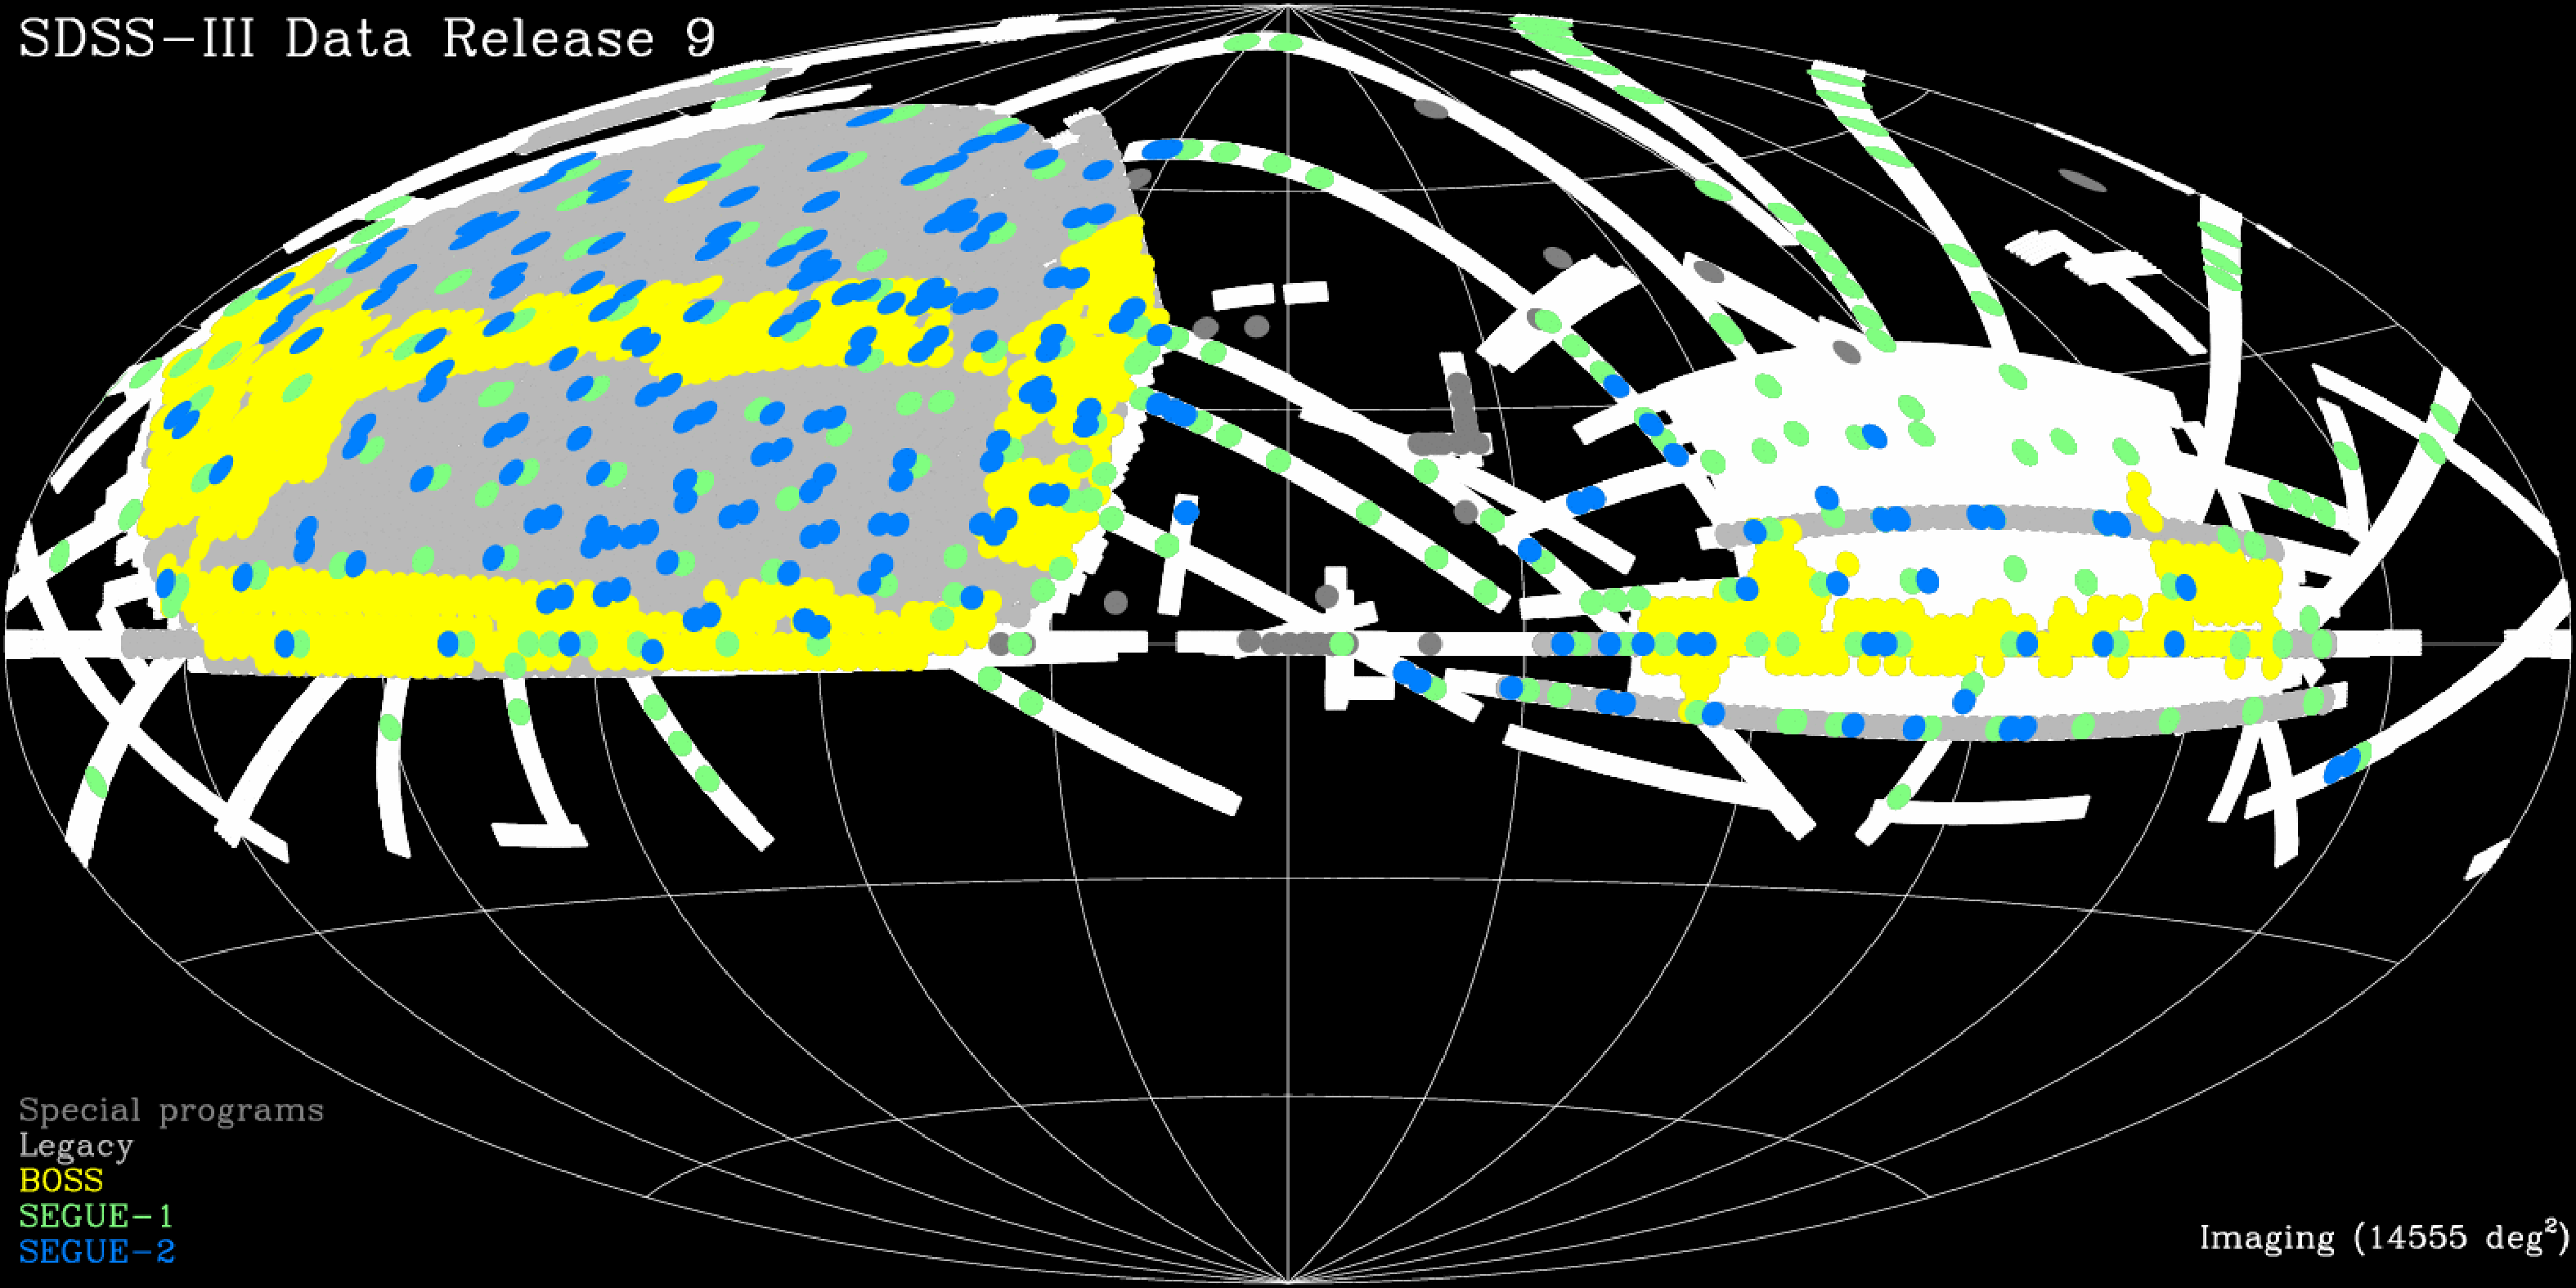
\includegraphics[width=12cm]{figuras/footprintsdss.pdf}
\caption{\textit{Footprint do SDSS-III em coordenadas equatoriais, para os dados lançados até o data release 9 (DR9). Os dados do BOSS estão representados pela cor amarela no mapa.}}
\label{fig:footprintsdss}
\end{center}
\end{figure}
\vspace{0.5cm}

\section{Dark Energy Survey}

O DES \cite{2005astro.ph.10346T} é um levantamento fotométrico que cobre  cerca de 5000 graus\textsuperscript{2} do hemisfério sul Galáctico. O projeto tem como principal objetivo melhor caracterizar o componente da energia escura, responsável pela expansão acelerada do Universo. \par
As observações são possíveis através da Dark Energy Camera (DECam), câmera CCD de 3 graus\textsuperscript{2} montada no foco primário do telescópio Blanco, de 4 metros, que fica localizado no Cerro Tololo Inter-American Observatory (CTIO) \cite{2015AJ....150..150F}. Na figura \ref{fig:footprintdes}\footnote{Créditos da imagem: Apresentação Josh Frieman DES-PAC Janeiro de 2014} mostramos a área do céu, que esperamos ser imageada ao longo  das observações do DES. \par

Os principais componentes da DECam, são uma câmera óptica CCD de 519 megapixels, um detector  óptico de campo largo (2.2 graus de visão de campo) e um sistema de filtros de 5 bandas grizY. Mostramos na figura \ref{fig:passbands}\footnote{Créditos da imagem: CTIO/NOAO/AURA/NSF} as funções de transmissão desses filtros. O plano focal da câmera consiste de sessenta e dois CCDs (0.27$''$/pixel), arranjados em um hexágono, cobrindo uma área de imageamento de 3 graus\textsuperscript{2}. \par 

As observações do DES começaram em agosto de 2013, o levantamento de dados será completado após 525 noites de observação, ao longo de cinco anos. Espera-se atingir os limites em magnitude de: g = 24.6, r = 24.1, i = 24.3 e z = 23.9. Estes são limites de 10$\sigma$ em $1.5''$ de abertura, assumindo um seeing de 0.9''.
As imagens produzidas pela DECam são reduzidas pelo grupo DES Data Management (DESDM), que desenvolveu um algoritimo para o processamento de dados, desde exposições únicas e correções instrumentais até a calibração de imagens co-adicionadas. \par
Neste trabalho nós usamos dados do primeiro e segundo ano do DES. Especificamente os catálogos co-adicionados  dos releases internos Y1A1 (referente ao ano 1) e Y2Q1 (referente a dados prévios do ano 2). Para maiores detalhes e referências sobre a redução de dados  do DESDM veja, \cite{2011arXiv1109.6741S,2012SPIE.8451E..0DM}. 
Para selecionarmos uma amostra estelar, usamos os parâmetros dados pelo Sextractor FLAGS, SPREAD MODEL e magnitudes PSF \cite{1996A&AS..117..393B,2012ApJ...757...83D}.
Os critérios que usamos para garantir a qualidade da fonte foram FLAGS $\le$ 3, sobre os três filtros  g r i. Também selecionamos magnitudes entre 17mag e 23mag, para cortarmos fontes muito brilhantes que podem saturar a imagem e fontes com espúrias. 
  Para selecionarmos uma amostra pura de estrelas, usamos o SPREAD MODEL na banda i como separador estrela/galáxia, selecionamos fontes do catálogo com $ |SPREAD \quad MODEL \quad i | \quad \le 0.003$, que são mais consistentes com fontes pontuais.    
Para evitar fontes pontuais com cores extremas (incluindo anãs vermelhas do disco Galáctico) também fizemos um corte em cor de  $-0.5 \le g-r \le 1.2$.



\begin{figure}[h]
\begin{center}
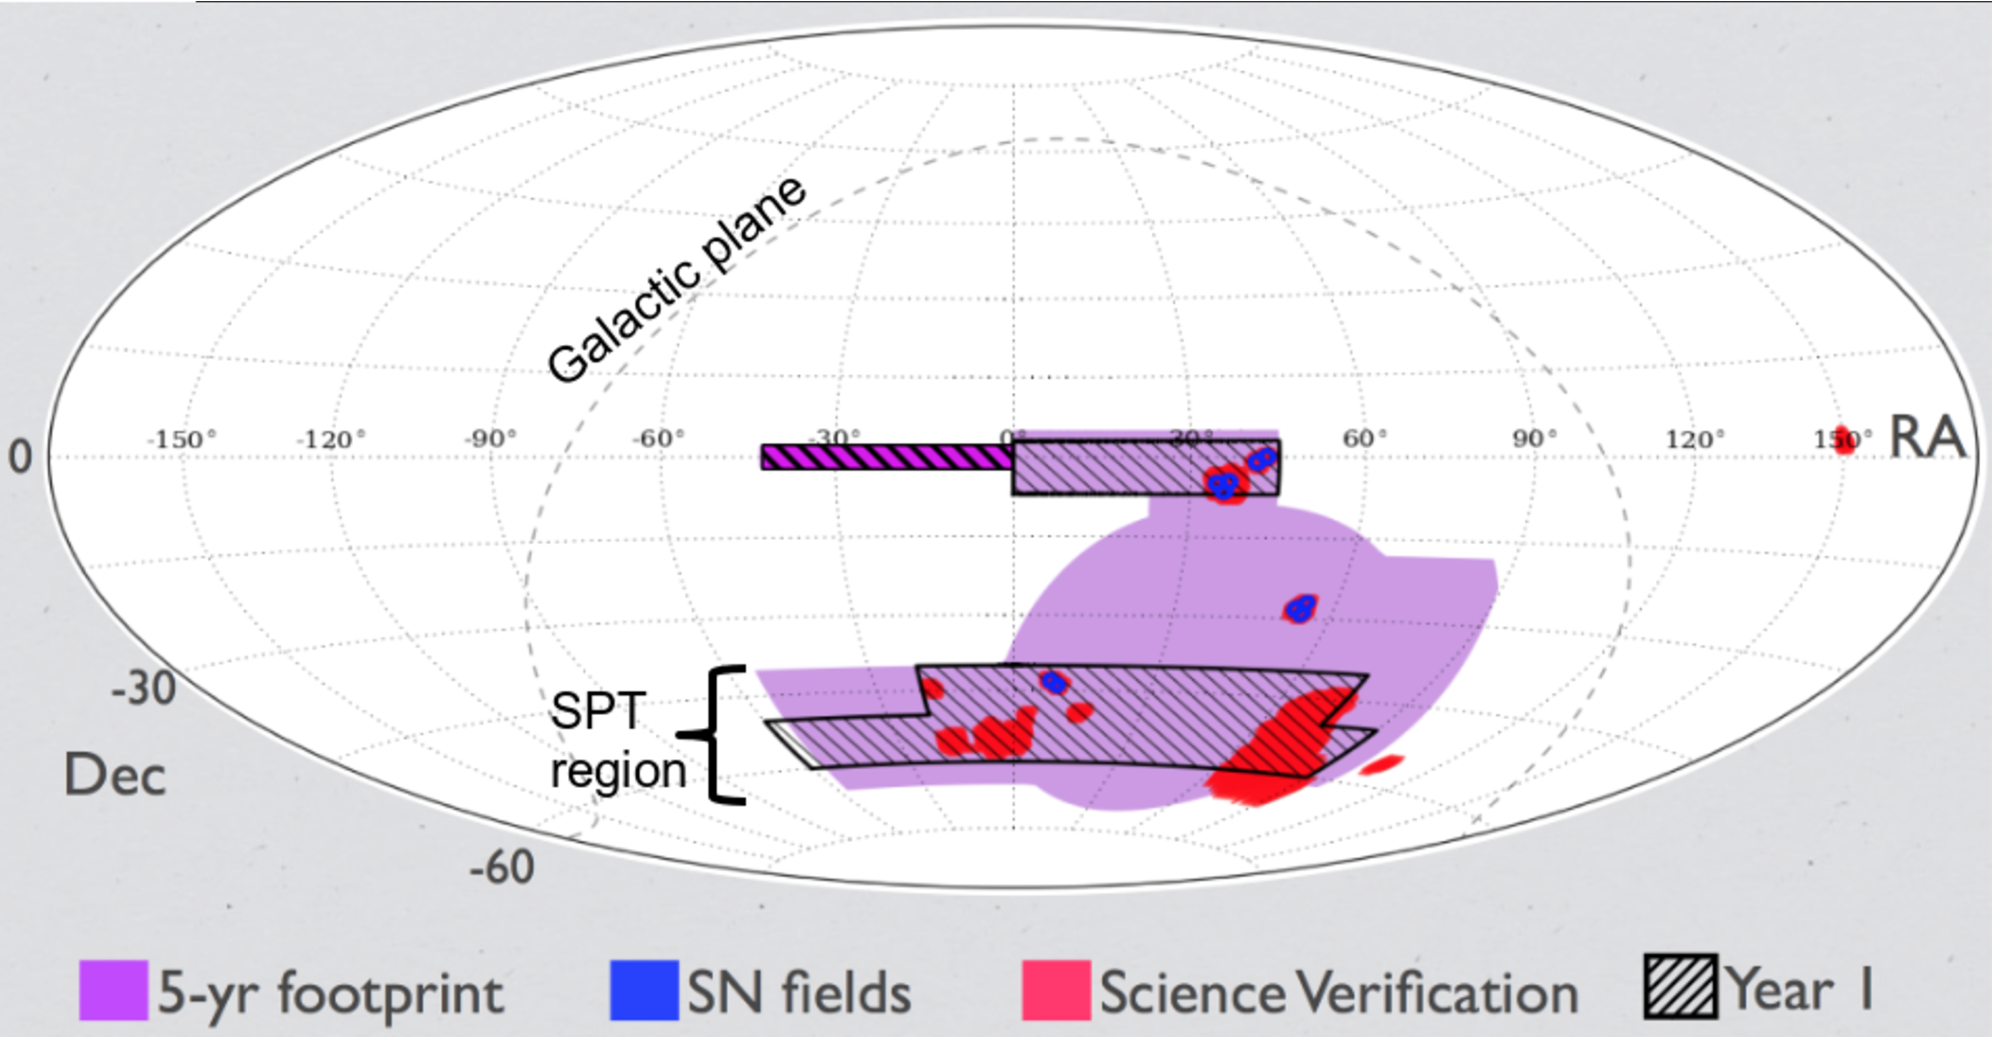
\includegraphics[width=12cm]{figuras/footprintdes.pdf}
\caption{\textit{Footprint do DES em coordenadas equatoriais, área lilás representa a área total a ser coberta pelo DES, as áreas em azul representam filtros de super nova, áreas em rosa representão dados de verificaçao e as áreas rachuradas representam os dados cobertos pelo ano 1.}}
\label{fig:footprintdes}
\end{center}
\end{figure}
\vspace{0.5cm}

\begin{figure}[h]
\begin{center}
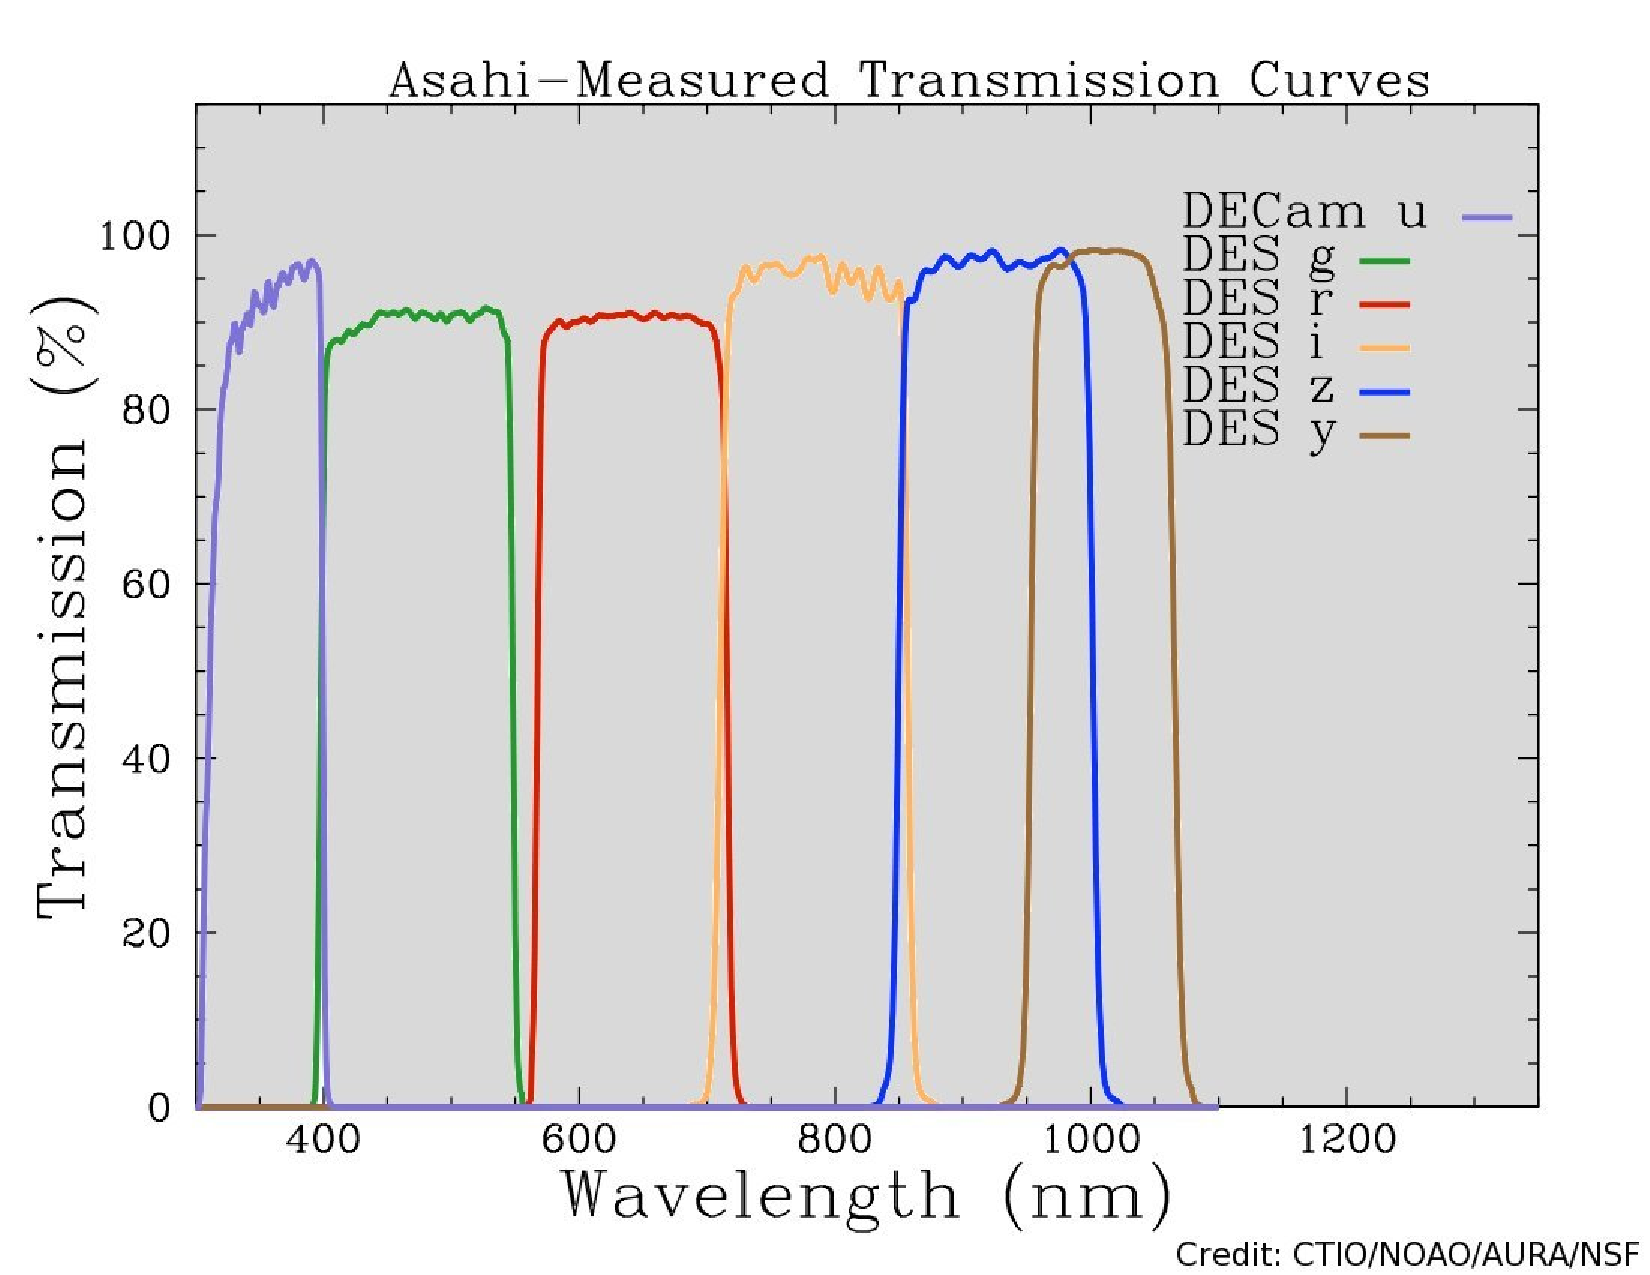
\includegraphics[width=12cm]{figuras/passbands.pdf}
\caption{\textit{Transmissão medida para os filtros ugrizY do DES. }}
\label{fig:passbands}
\end{center}
\end{figure}
\vspace{0.5cm}



\chapter{Matched Filter}
% ---
O Matched Filter (MF) é uma técnica com diversas aplicações para processamento de sinais. No contexto da astronomia, vem sendo usado principalmente para detectar Populações Estelares Simples (SSP)s de baixa densidade em dados de imageamento \cite{2012ASPC..458..219G,2009AAS...21344217D}. Aqui usamos o MF como parte do algoritmo SparSEx para detecção dos satélites da VL e também de correntes estelares seguindo o trabalho de \cite{2011MNRAS.416..393B}. \par
O número de estrelas como função da posição no céu ($\alpha$,$\delta$)  e também da cor $(c)$ e magnitude $(m)$ pode ser escrito como:
\begin{equation} \label{eq:densnum}
N(\alpha,\delta,c,m) = N_{cl}(\alpha,\delta,c,m)+ N_{bg} (\alpha,\delta,c,m) 
\end{equation}
O primeiro termo no lado direito da equação corresponde à contribuição do sistema estelar que queremos descobrir $(cl)$, enquanto que o segundo termo corresponde à contribuição das estrelas de campo $(bg)$. Ambas as quantidades podem ser separadas em um termo de normalização e uma função de distribuição de probabilidade (PDF). Por definição, uma SSP é descrita por uma única distribuição no espaço de cor magnitude, mas a densidade numérica das suas estrelas pode variar em função da sua posição. Sendo assim podemos escrever:
\begin{equation}
n_{cl}(\alpha,\delta,c,m) = \xi_{cl}(\alpha,\delta)f_{cl} (c,m) 
\end{equation}

Onde $\xi_{cl}$ e $f_{cl}$ são respectivamente, a normalização do número de estrelas da SSP e sua PDF, no espaço do CMD. Para as estrelas de campo da nossa Galáxia, sabemos que ambos o número de estrelas e o CMD variam como função da posição através do céu. Sendo assim, escrevemos:
\begin{equation}
n_{bg}(\alpha,\delta,c,m) = \xi_{bg}(\alpha,\delta)f_{bg} (\alpha,\delta,c,m) 
\end{equation}
Note que as funções $f_{cl}$ e $f_{bg}$ são funções estatísticas que descrevem a probabilidade de uma estrela, randomicamente selecionada, pertencer à SSP ou ao campo,  dado sua posição no CMD. \\ 
Considerando todas as premissas citadas a cima,  a equação \ref{eq:densnum} pode ser reescrita da forma:

\begin{equation} \label{eq:numdens2}
N(\alpha,\delta,c,m) = \xi_{cl}(\alpha,\delta)f_{cl} (c,m) + \xi_{bg}(\alpha,\delta)f_{bg} (\alpha,\delta,c,m) 
\end{equation}
 
Nós construímos as PDFs, $f_{cl}$ e $f_{bg}$, por meio de diagramas de Hess em bins de 0.01 em cor e 0.1 em magnitude. Por questões práticas de notação, vamos nos referir ao CMD usando o índice j. O céu também é dividido em bins que escolhemos ter uma área de 1x1 $arcmin^2$. Os bins no espaço de posição são representados pelo índice i. Podemos então, transformar as equações  $n_{cl}$ e $n_{bg}$ em funções discretas.

\begin{equation}
n(i,j) = \xi_{cl}(i)f_{cl} (j) + \xi_{bg}(i)f_{bg} (i,j) 
\end{equation}

O lado esquerdo representa o número observado de estrelas em uma dada posição do céu e do CMD. Se o número de estrelas observadas no catálogo é N(i,j), podemos então construir a variância entre este número e o número esperado da SSP para cada bin espacial: 

\begin{equation}
S^2(i) = \sum\limits_{j}\frac{[N(i,j)  - \xi_{cl}(i) f_{cl}(j)  - \xi_{bg}(i) f_{bg}(i,j)]^2}{\xi_{bg}(i)f_{bg}(i,j)}
\end{equation}

O termo do denominador expressa a flutuação poissonica esperada na contagem de estrelas, que, por simplicidade, nós tomamos por ser dominada pelas estrelas de campo. Minimizando essa equação e resolvendo para $\xi_{cl}(i)$,  temos o número de estrelas observadas em cada direção no céu que, de acordo com o modelo dado pela equação \ref{eq:numdens2}, são mais consistentes com o modelo de SSP.

\begin{equation}
\xi_{cl}(i) = \frac{\sum\limits_{j}N(i,j)f_{cl}(j)/f_{bg}(i,j)}{\sum\limits_{j}f_{cl}^2(j)/f_{bg}(i,j)} - \frac{\xi_{bg}(i)}{\sum\limits_{j}f_{cl}^2(j)/f_{bg}(i,j)}
\end{equation}

No final, como saída do código, temos um mapa de densidade estelar fornecida pela matriz  $\xi_{cl}(i)$ . 
Em prática, nós modelamos a PDF do campo, $f_{bg}(i,j)$, usando amostras tiradas diretamente do catalogo estelar onde se faz a busca. Nós fazemos isso sob a suposição de que a contaminação pelas SSPs a serem detectadas são insignificantes. Para a PDF da SSP, nós fazemos uso de simulações baseadas em modelos de evolução estelar que será explicada adiante. 

\chapter{Simulações}


Como explicado na sessão anterior, o MF funciona como uma modelagem do número de estrelas esperado,  em cada direção do céu, para as estrelas de campo e de uma SSP. Para fazermos uma busca por satélites da Galáxia, de cujas características não temos informação prévia,  necessitamos simular uma grade de diferentes SSPs. Para essa tarefa usamos o código GenCMD. O  GenCMD usa isócronas de PADOVA \cite{2012MNRAS.427..127B} e randomicamente seleciona massas estelares seguindo uma função de massa incial (IMF) pré-definida. Nós decidimos adotar uma IMF do tipo Kroupa \cite{2001MNRAS.322..231K} nas simulações. Para cada massa estelar, interpolamos as isócronas para obter as magnitudes absolutas nos filtros desejados.\par
Para transformar essas magnitudes absolutas (M) em magnitudes aparentes (m) procedemos da seguinte maneira, esse processo é feito para cada um dos filtros:
Primeiro, aplicamos à magnitude absoluta erros fotométricos gaussianos err(M), usando incertezas em magnitude correspondentes ao SDSS e ao DES. 
	\begin{equation}
	M\textsubscript{e} = M + err(M) 
	\end{equation}
Segundo, adicionamos M\textsubscript{e} ao módulo de distância, correspondente a uma distância d[pc] adotada.
	\begin{equation}
	(m)\textsubscript{0} = 5*log\textsubscript{10} d  -5 + M\textsubscript{e}
	\end{equation}

Terceiro, aplicamos o avermelhamento, A\textsubscript{$\nu$}, de acordo com os mapas de poeira de Schlegel \cite{1998ApJ...500..525S}.
	\begin{equation}
	m =  (m)\textsubscript{0} + A\textsubscript{$\nu$}
	\end{equation}			
						
Por fim, as posições no céu foram simuladas  de acordo com o perfil de densidade Hubble modificado \cite{1972ApJ...175..627R}. \par

Nós usamos cada um desses modelos simulados como entrada na aplicação do MF. A grade descrita na tabela \ref{tab:1} foi usada nos dados do BOSS, com o objetivo de detectar, principalmente, aglomerados estelares. Enquanto que a grade descrita na tabela \ref{tab:2} foi usada em outras áreas do SDSS, com o propósito de recuperar galáxias anãs e aglomerados conhecidos.

\begin{table}[h]
\caption{\emph{Grade de Parâmetros usada simulações de SSPs, para busca de aglomerados estelares no BOSS. A grade inclui um total de 1485 modelos.}} 
\centering
\begin{tabular}{cccc}
\hline
Parâmetros & Limite inferior & Limite superior & passos \\
\hline
\hline
Log($\tau$) & 9.0 & 10.1 & 0.1 \\
$Z$ & 0.001 & 0.019 & 0.002 \\
$d (kpc)$ & 10 & 40 & 2 \\
\hline
\end{tabular}
\label{tab:1}
\end{table}


\begin{table}[h]
\caption{\emph{ Grade de parâmetros usados na simulação de SSPs para procura de satélites no SDSS e outros surveys. A grade inclui um total de 228 modelos.}}
\centering
\begin{tabular}{cccc}
\hline
Parâmetros & Limite inferior & Limite superior & passos \\
\hline
\hline
Log($\tau$) & 9.0 & 10.2 & 0.3 \\
$Z$ & 0.0002 & 0.001 & 0.007 \\
$d (kpc)$ & 10 & 200 & 10 \\
\hline
\end{tabular}
\label{tab:2}
\end{table}




\chapter{Identificação dos candidatos}
Após a aplicação do MF em cada SSP simulada, temos que analisar todos os mapas de densidade resultantes em busca dos candidatos a satélite da VL. Porém o número de mapas pode ser muito grande para fazermos uma busca visual. Por exemplo, a grade representada na tabela \ref{tab:1} resulta em 1485 mapas para serem analisados. E mesmo após o processo do MF, a análise visual pode deixar “escapar” alguns candidatos, por terem sinal baixo.  \par
Para solucionar esse problema usamos o código SExtractor, \cite{1996A&AS..117..393B}, que sistematicamente procura por picos de densidade em cada um dos mapas.
Para cada mapa de densidade, correspondente a uma  dada SSP usada no MF, aplicamos kernels gaussianos de convolução que variam em tamanhos de $ \{ \sigma = 0'\quad (sem convolução)\quad à\quad  \sigma = 9'\}$, para podermos realçar estruturas com escalas típicas de aglomerados globulares e galáxias anãs. Essa suavização é feita como uma ferramenta do próprio SExtractor. \par
Para cada um dos mapas convoluídos, o  SExtractor detecta picos de densidade, e os coloca em uma lista, correspondente ao tamanho do kernel utilizado. Note que um mesmo objeto pode ser detectado  em mapas de diferentes SSPs, ou seja, o mesmo objeto pode ser detectado em mais de um mapa analisado pelo SExtractor. Portanto, é necessário verificar as ocorrências de repetições nas listas dadas pelo SExtractor. Ao fazer essa verificação contabilizamos o número de vezes que certo objeto foi detectado. Em outras palavras, determinamos o número de  modelos que detectou o mesmo objeto pelo MF em todos os N modelos simulados.
É a partir desse número de repetições,  que organizamos o nosso arquivo final com os candidatos por ordem de importância. Quanto maior o número de  repetições, mais provável que o candidato seja um sistema real. \par
As listas finais organizadas por repetição serão então o resultado final do algorítimo SparSEx. Para uma melhor compreensão do método, mostramos na figura \ref{fig:fluxo} um fluxograma do processo de simulações $\Rightarrow$ MF  $\Rightarrow$ determinação dos candidatos. \par

Nem todos os objetos detectados pelo SExtractor são reais. Existem, é claro, defeitos no catálogo, objetos extensos e complexos (como galáxias próximas) ou flutuações na contagem de estrelas de campo que podem ser detectados como falsos positivos. Para termos certeza de que os candidatos são mesmo reais, precisamos checar se o seus CMDs e seus perfis densidade são consistentes com os de uma população estelar. Este procedimento é o  último passo na busca por subestruturas da Galáxia.  


\begin{figure}[h]
\begin{center}
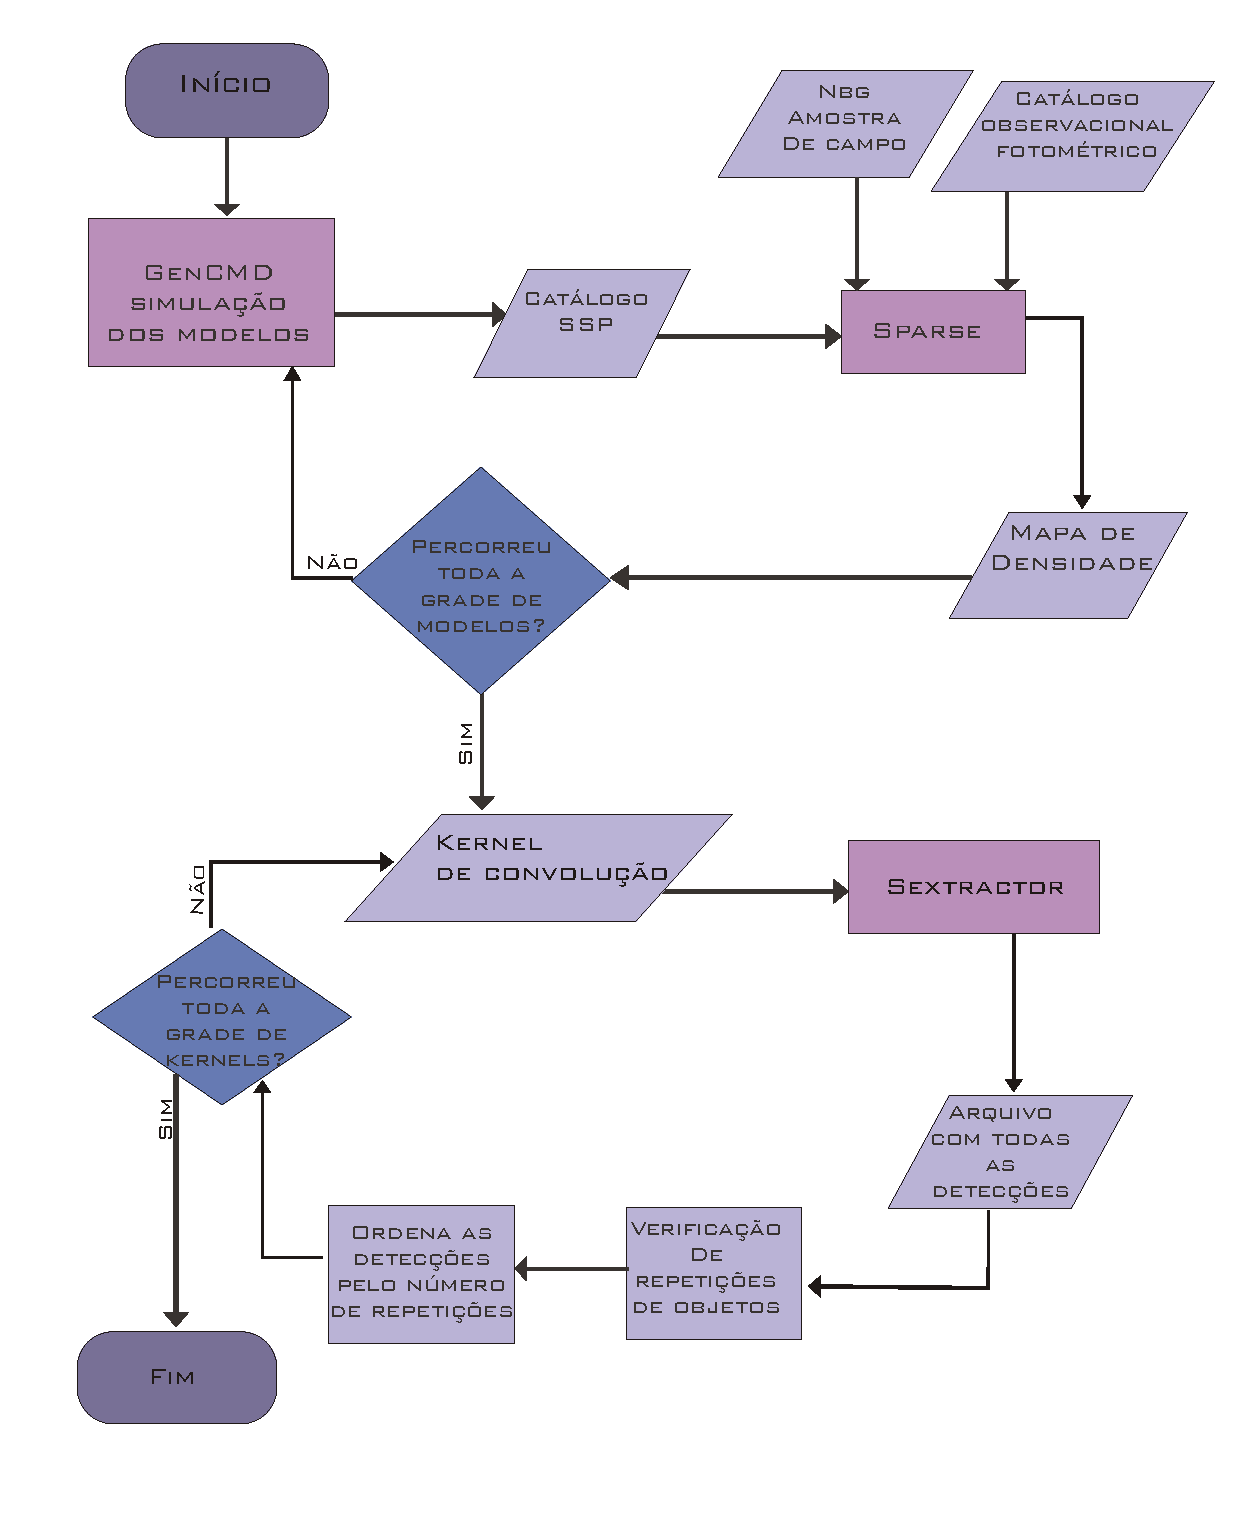
\includegraphics[width=12cm]{figuras/fluxogramaSparsex.pdf}
\caption{\textit{Fluxograma do algorítimo SparSEx: primeiramente é simulado um  modelo de SSP, este serve como entrada do MF, juntamente com o catálogo observacional e uma amostra de campo. O processamento do MF  gera, como resultado, uma mapa de densidade com as estrelas consistentes com a SSP. Após aplicarmos o MF a todos os modelos, aplica-se um kernel de convolução gaussiana em todos os mapas resultantes do MF. Após este, o SExtractor faz a busca por picos de densidades nos mapas, provendo uma lista de candidatos. Por fim, faz-se a verificação de repetições na lista e o ordenamento dos objetos pelo número de repetições. Após a grade de kernels ser completada, o SparSEx termina.}}
\label{fig:fluxo}
\end{center}
\end{figure}
\vspace{0.5cm}

% ----------------------------------------------------------
% PARTE
% ----------------------------------------------------------
\part{Desenvolvimento do trabalho}
% ----------------------------------------------------------

% ---
% primeiro capitulo de Resultados
% ---
\chapter{Validação}
\label{cha:validacao}
% ---
Para validar o SparSEx, usamos os dados do SDSS, como teste para encontrar galáxias anãs e aglomerados globulares conhecidos. Aplicamos o método, em média, em áreas de 9 graus\textsuperscript{2}, em torno desses alvos. Todos os sistemas que foram usados como teste, foram recuperados como candidatos muito prováveis a populações estelares, ou seja, obtiveram um  alto ranqueamento na lista final de candidatos resultante do SparSEx. Mostramos na tabela \ref{tab:3} os sistemas recuperados e seus parâmetros resultantes da aplicação do SparSEx.

\begin{table}[h]
\caption{\emph{Objetos conhecidos detectados pelo SparSEx, e seus parâmetros de saída: $N^{\underline{o}}$ de modelos, usados pelo MF, com que se recuperou a estrutura; Ranqueamento:  classificação  baseada em $N^{\underline{o}}$ de modelos; Convolução (FWHM-SE): parâmetro do Sextractor usado como a FWHM da convolução gaussiana, para suavizar os mapas de densidade, ao qual os parâmetros anteriores (Ranqueamento e  $N^{\underline{o}}$ de modelos) se referem; $N^{\underline{o}}$ de estrelas/pixel: densidade do objeto detectado.}}
\centering
\begin{tabular}{p{3.0cm}p{2.0cm}p{2.5cm}p{2.8cm}p{2.8cm}}
\hline
Galáxias Anãs & $N^{\underline{o}}$ de modelos & Ranqueamento & Convolução FWHM-SE(pixels) & $N^{\underline{o}}$ de estrelas/pixel  \\
\hline
\hline
Canes Venatici I & 106 & 1 & 5 & $\approx$ 14.0 \\
Canes Venatici II & 16 & 1 & 1.5 & $\approx$ 14.0 \\
Coma & 28 & 1 & 5.0 & $\approx$ 15.0 \\
Hercules & 10 & 1 & 2.5 & $\approx$ 42.5 \\
Leo IV & 30 & 3 & 3.0 & $\approx$ 10.5 \\
Leo V & 11 & 3 & 4.0 & $\approx$ 7.0 \\
Leo T & 84 & 1 & 2.5 & $\approx$ 9.5 \\
Segue I & 16 & 3 & 4.0 & $\approx$ 11.5 \\
Segue II & 10 & 2 & 4.0 & $\approx$ 7.0 \\
Ursa Maior I & 17 & 3 & 3.0 & $\approx$ 6.3 \\
Willman I & 81 & 1 & 5.0 & $\approx$ 6.5 \\
\hline
Aglomerados globulares \\
\hline
\hline
Balbinot I & 510 & 1 & Sem Conv. & $\approx$ 15.8 \\
Koposov I & 62 & 1 & Sem Conv. & $\approx$ 13.5 \\
Koposov II & 13 & 1 & 1.5 & $\approx$ 26.6 \\
Palomar 13 & 1192 & 1 & Sem Conv & $\approx$ 17.0 \\
Segue 3 & 1071 & 1 & Sem Conv & $\approx$ 16.6 \\
Whiting I & 1154 & 1 & Sem Conv & $\approx$ 17.5 \\
\hline
\end{tabular}
\label{tab:3}
\end{table}

Além dos parâmetros mostrados na tabela \ref{tab:3}, a lista de parâmetros de saída do SparSEx também inclui as posições e eixo maior dos candidatos. No começo estávamos usando esses parâmetros para construir CMDs  automaticamente. Mas como podemos ver na figura \ref{fig:central}, a posição central do objeto Koposov II está um pouco deslocada. 

\begin{figure}[h]
\begin{center}
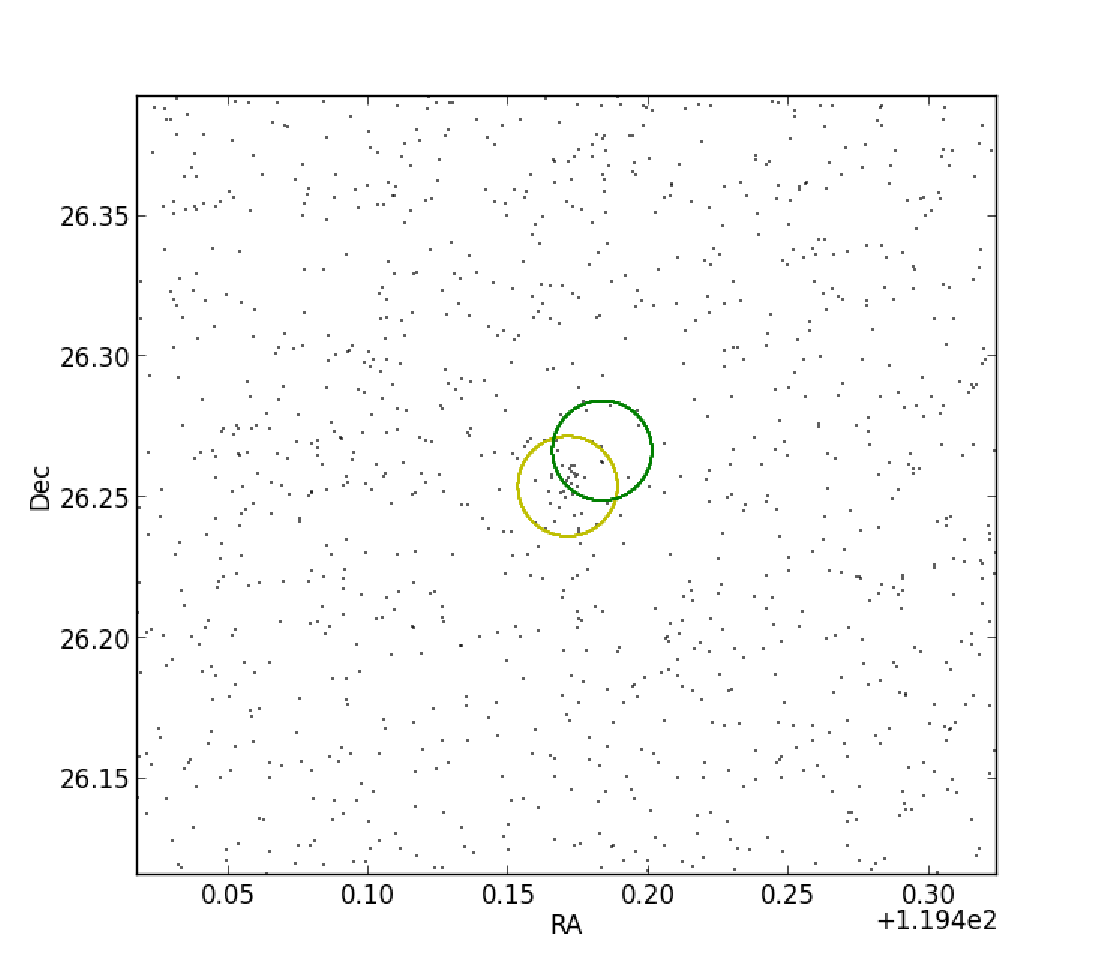
\includegraphics[width=12cm]{figuras/center.pdf}
\caption{\textit{Distribuição espacial de estrelas, em coordenada equatoriais, em torno de Koposov II. O círculo verde indica a posição do aglomerado dado pelo Sextractor. Nós ajustamos o centro do aglomerado, visualmente, e indicamos a nova posição pelo círculo amarelo. }}
\label{fig:central}
\end{center}
\end{figure}
\vspace{0.5cm}


Na sequência mostramos os resultados para duas galáxias anãs, Canes Venatici e Hercules, e para o aglomerado globular Koposov II. Primeiro mostramos nas figuras \ref{fig:denmapCVnI} ,\ref{fig:denmapHer} e \ref{fig:denmapKoII} os mapas de densidade resultantes da aplicação do MF, com um modelo que recuperou o objeto com o maior sinal. Podemos ver claramente nessas figuras as sobredensidades detectadas posteriormente pelo Sextractor. \par 
Após a detecção desses objetos nós plotamos os perfis de densidade e os ajustamos a um perfil de king \cite{1962AJ.....67..471K} para as três subestruturas, figuras \ref{fig:kingCVnI}, \ref{fig:kingHer} e \ref{fig:kingKoII}. Fizemos estes ajustes com o intuito de obter  seus raios de core e por fim, construir seus CMDs em uma área com dimensões próximas aos tamanhos dos objetos. Mostramos os CMD das subestruturas nas figuras \ref{fig:cmdCVnI}, \ref{fig:cmdHer} e \ref{fig:cmdKoII}. Os CMDs foram construídos dentro de um círculo com raio igual ao raio de core do objeto. Plotamos também, ao lado dos CMDs dos candidatos, as estrelas de campo de uma área próxima aos objetos. No CMD de Canes Venatici I, figura \ref{fig:cmdCVnI}, podemos ver o ramo de gigantes, o ramo horizontal e o turn off de estrelas. Todavia, para os CMDs de Hercules e Koposov II,  figuras \ref{fig:cmdHer} e \ref{fig:cmdKoII}, é preciso de uma análise mais cuidadosa para ver a consistência desses CMDs com os de uma população estelar. Estes CMDs são compatíveis com os dos artigos de descoberta de Hercules, Canes Venatici \cite{2007ApJ...654..897B} e  Koposov II \cite{2007ApJ...669..337K}.

\begin{figure}[H]
\begin{center}
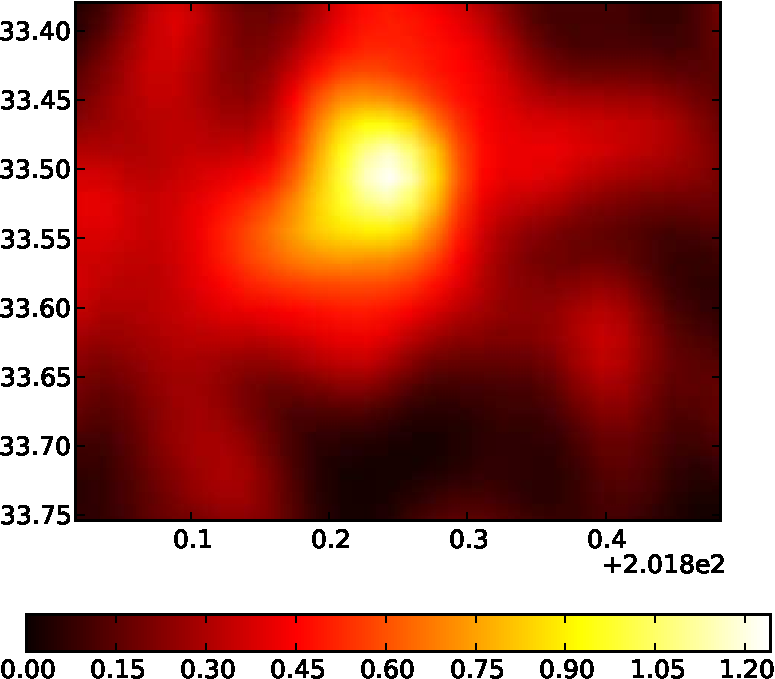
\includegraphics[width=12cm]{figuras/mapa_densityCVnI.pdf}
\caption{\textit{Mapa de densidade de Canes Venatici I, resultante da aplicação do MF com um modelo de: 10 kpc de distância, 9.9 $\Log anos$ e 0.001z. Este mapa foi suavizado com uma FWHM de $5'.0$ pelo Sextractor.}}
\label{fig:denmapCVnI}
\end{center}
\end{figure}
\vspace{0.5cm}

\begin{figure}[H]
\begin{center}
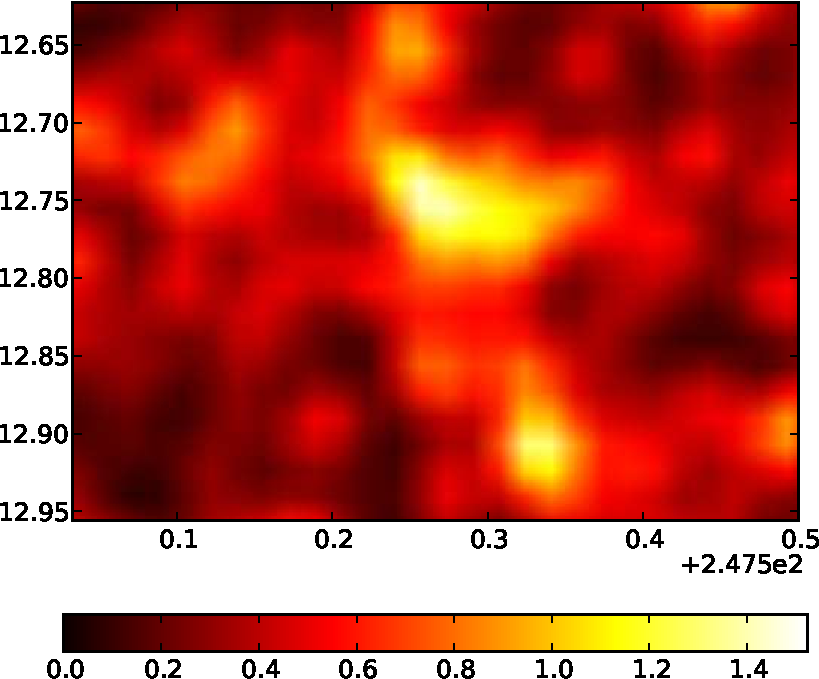
\includegraphics[width=12cm]{figuras/mapa_densityHer.pdf}
\caption{\textit{Mapa de densidade de Hercules, resultante da aplicação do MF com um modela de: 10 kpc de distância, 10.20 $Log anos$ e 0.001z. Este mapa está suavizado com um FWHM $2'.5$. Podemos ver que a sobredensidade de Hercules não é tão clara como a de Canes Venatici I. }}
\label{fig:denmapHer}
\end{center}
\end{figure}
\vspace{0.5cm}

\begin{figure}[H]
\begin{center}
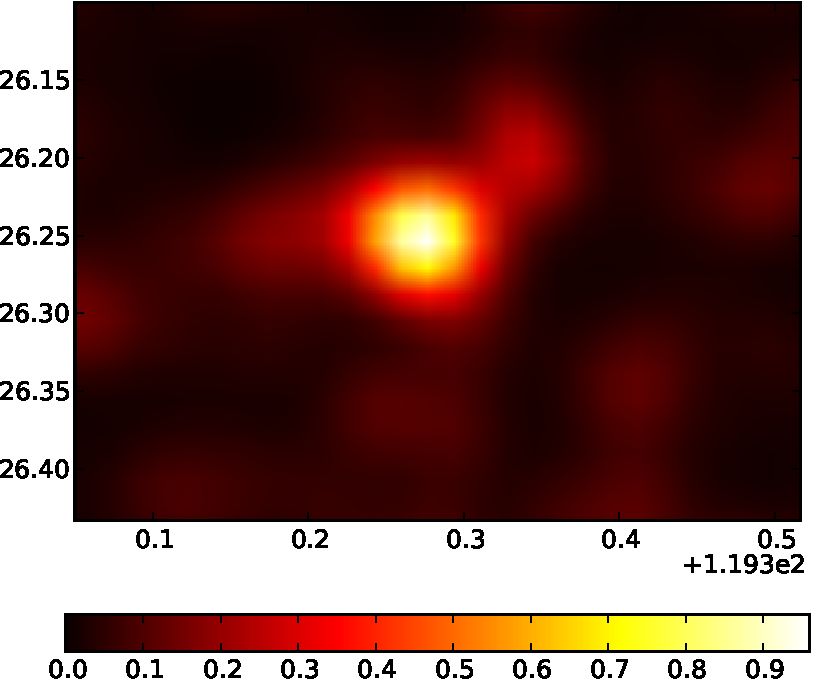
\includegraphics[width=12cm]{figuras/mapa_sparse_conv_Koposov2.pdf}
\caption{\textit{Mapa de densidade do aglomerado globular  Koposov II, resultante da aplicação do MF com um modela de: 170 kpc de distância, 9.30 $Log anos$ e 0.002z. Este mapa está suavizado com um FWHM $1'.5$. Podemos ver que a sobredensidade compacta  é consistente com a de um aglomerado globular. }}
\label{fig:denmapKoII}
\end{center}
\end{figure}
\vspace{0.5cm}

\begin{figure}[H]
\begin{center}
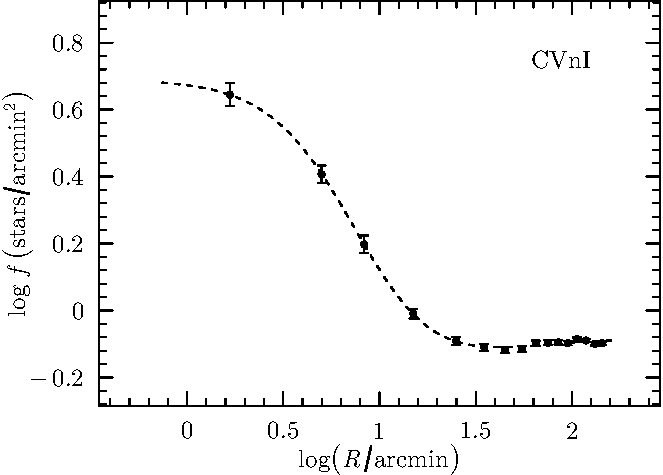
\includegraphics[width=12cm]{figuras/King_profile_CVnI.pdf}
\caption{\textit{Perfil de densidade radial para Canes Venatici I. A linha tracejada representa o melhor ajuste para o perfil de King.  Desse ajuste obtivemos um raio de core de $ r\textsubscript{c} = 4'.86 \pm 0'.07$}}
\label{fig:kingCVnI}
\end{center}
\end{figure}
\vspace{0.5cm}

\begin{figure}[H]
\begin{center}
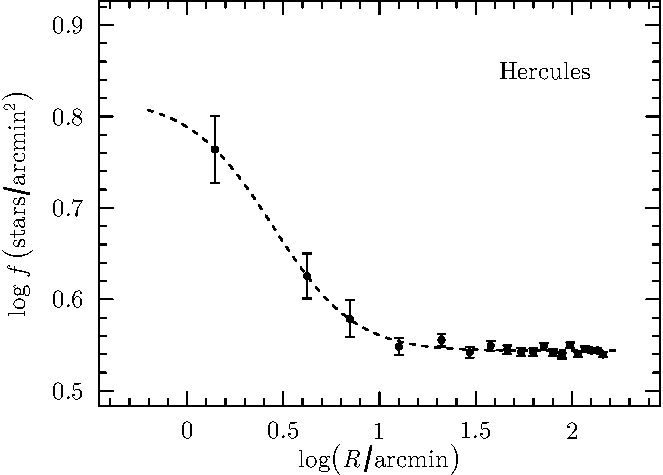
\includegraphics[width=12cm]{figuras/King_profile_Her.pdf}
\caption{\textit{Perfil de densidade radial para a galáxia anã Hercules. A linha tracejada representa o melhor ajuste para o perfil de King.  Desse ajuste obtivemos um raio de core de $ r\textsubscript{c} = 2'.41 \pm 0'.16$}}
\label{fig:kingHer}
\end{center}
\end{figure}
\vspace{0.5cm}

\begin{figure}[H]
\begin{center}
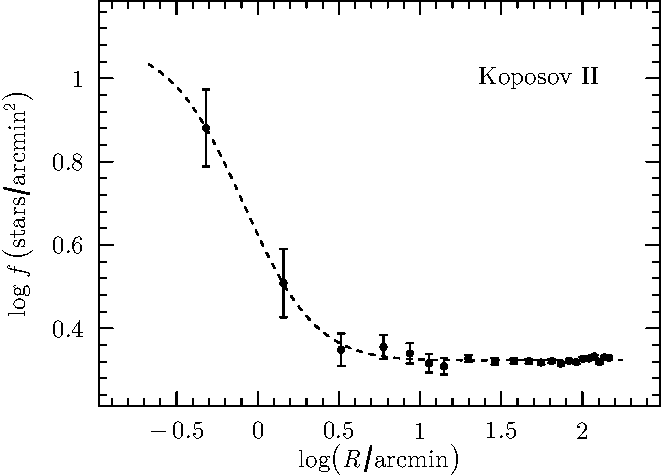
\includegraphics[width=12cm]{figuras/King_profile_Koposov2.pdf}
\caption{\textit{Perfil de densidade radial para o aglomerado globular Koposov II. A linha tracejada representa o melhor ajuste para o perfil de King.  Desse ajuste obtivemos um raio de core de $ r\textsubscript{c} = 0'.53 \pm 0'.05$}}
\label{fig:kingKoII}
\end{center}
\end{figure}
\vspace{0.5cm}

\begin{figure}[H]
\begin{center}
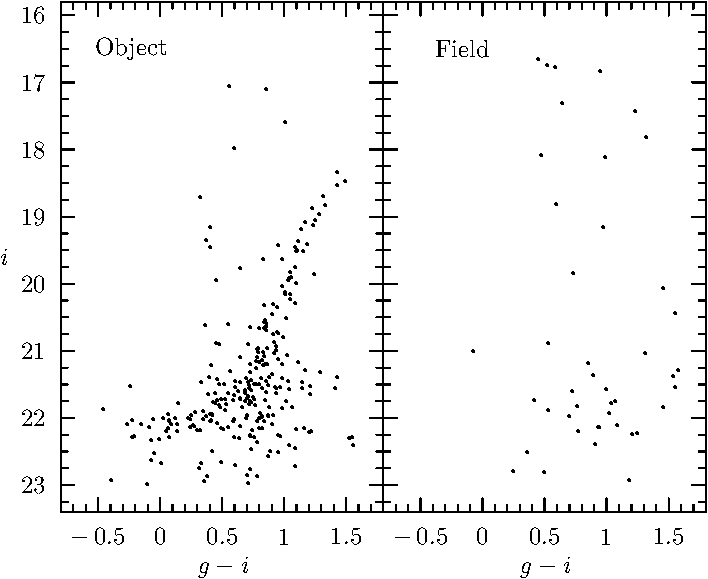
\includegraphics[width=12cm]{figuras/cmdCVnI_ixgi.pdf}
\caption{\textit{Painel esquerdo: CMD de Canes Venatici I. Podemos ver, claramente, o seu ramo de gigante, o seu ramo horizontal e o turn off de estrelas; Painel direito: CMD das estrelas de campo próximas a Canes Venatici I. Vemos que a população estelar desta galáxia é bem evidente em  relação à população de campo. }}
\label{fig:cmdCVnI}
\end{center}
\end{figure}
\vspace{0.5cm}

\begin{figure}[H]
\begin{center}
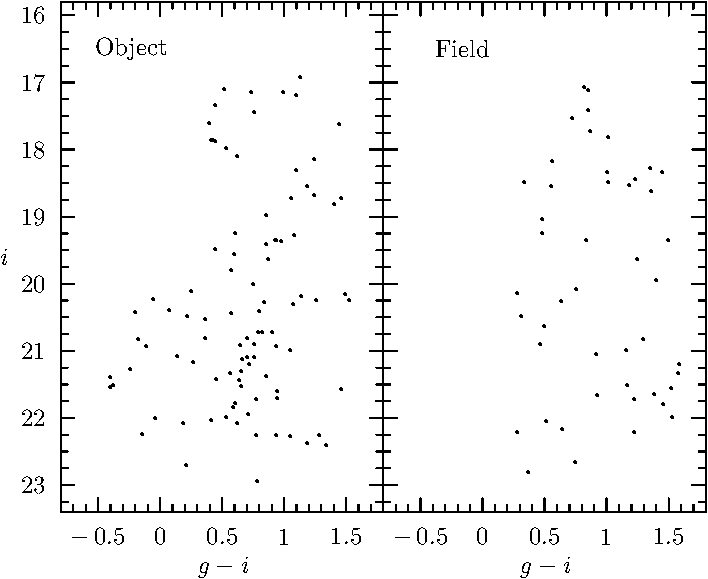
\includegraphics[width=12cm]{figuras/cmdHer_ixgi.pdf}
\caption{\textit{Painel esquerdo: CMD de Hercules. Não é muito fácil ver as características de uma SSP nesse CMD; Painel direito: CMD das estrelas de campo próximas a Hercules. Nesse caso o CMD do objeto não difere muito em densidade do CMD do campo, uma descontaminação das estrelas de campo é recomendável para essa situação. }}
\label{fig:cmdHer}
\end{center}
\end{figure}
\vspace{0.5cm}

\begin{figure}[H]
\begin{center}
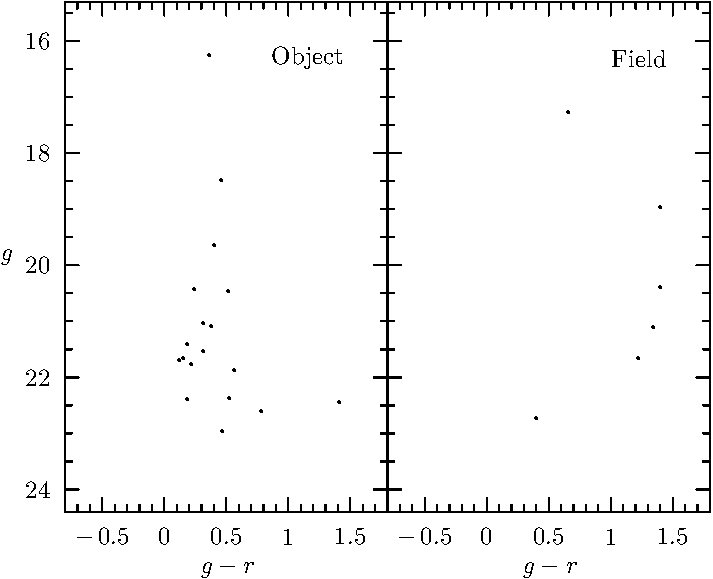
\includegraphics[width=12cm]{figuras/cmdKoposov2_rxgr.pdf}
\caption{\textit{Painel esquerdo: CMD do aglomerado globular  Koposov II. Não é muito fácil ver as características de uma SSP nesse CMD; Painel direito: CMD das estrelas de campo próximas a Koposov II. Nesse caso o CMD não difere muito em densidade do CMD do campo. Uma descontaminação das estrelas de campo é mais complexa nesse caso, pois a amostra de estrelas é pequena para aplicação de métodos estatísticos. Seria necessário observações de follow-up para aumentarmos a amostra de estrelas e confirmarmos este como população estelar \cite{2007ApJ...669..337K}}}

\label{fig:cmdKoII}
\end{center}
\end{figure}
\vspace{0.5cm}

Outra validação muito importante do SparSEx é recuperação da corrente estelar da galáxia anã de Sagitário. Ao aplicar o SparSEx em uma área de 40x40 graus\textsuperscript{2} no footprint do BOSS, especificamente na área em torno da corrente estelar de sagitário, obtemos uma lista com as posição de todos os candidatos a SSP nessa área. Ao plotar todas as posições dessa lista observamos algo curioso. Pela figura \ref{fig:sagstream}, podemos ver claramente que a maioria dos candidatos delineam a estrutura da cauda da anã de sagitário. Uma vantagem desse método para detecção de correntes estelares é que ele é composto de várias SSPs com diferentes distâncias e metalicidades, e usualmente as correntes estelares têm uma variação em distância e/ou populações ao longo de usa extensão. Na figura \ref{fig:sagstream} também podemos observar na parte superior do gráfico, detecções no entorno da galáxia de Andrômeda (M31) e da galáxia Triângulo (M33).


\begin{figure}[H]
\begin{center}
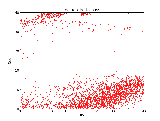
\includegraphics[width=12cm]{figuras/sagitarius-stream.pdf}
\caption{\textit{Plot da posição dos candidatos encontrados pelo SparSEx em parte do footprint do BOSS. Vemos que os candidatos formam a estrutura da corrente estelar da galáxia anã de  Sagitário \cite{2001ApJ...547L.133I}, no canto inferior do gráfico. A concentração de pontos na parte superior do gráfico  é devida às galáxias do grupo local M31 e M33, visto que M31 tem um grande sistema de galáxias satélites. }}
\label{fig:sagstream}
\end{center}
\end{figure}
\vspace{0.5cm}

% ---
\chapter{Aplicação nos dados do DES}
\label{cha:dadosdes}
% ---
Nos últimos dois anos, tralhamos juntamente com o grupo de Milky Way (MW) do Dark Energy Survey na busca de subestruturas da VL. Para essa tarefa, utilizamos três diferentes métodos para detecção de populações estelares. Um deles é o SparSEx. Para detalhes dos outros métodos de detecção veja: \cite{2015arXiv150803622T}. Em março desse ano publicamos a descoberta de  8  novos satélites da VL \cite{2015ApJ...807...50B} e em agosto publicamos a descoberta de outros 8 satélites \cite{2015arXiv150803622T}. Mostramos na tabela \ref{tab:des} as posições equatoriais e as principais características dessas novas estruturas. \par
Esses objetos foram obtidos de uma união dos candidatos indicados pelos três métodos.  Comparamos as posições dos candidatos encontrados com listas de aglomerados e galáxias anãs conhecidas \cite{1998AJ....116.3040G,2012AJ....144....4M} e também com listas de objetos que podem produzir falsos positivos, como galáxias próximas ou aglomerados de galáxias.
A caracterização dos objetos foi determinada por uma analise de verossimilhança de Markov Chain Monte Carlo (MCMC), usando isócronas de PADOVA\cite{2012MNRAS.427..127B} . Os melhores valores ajustados e incertezas são determinadas pelos picos da distribuição posterior e os 90$\%$ maiores intervalos de densidade da posterior. 


\begin{table}[h]
\caption{\emph{Características dos novos satélites da Via Láctea descobertos com os dados no ano1 (Y1A1) e do ano2 (Y2Q1) do DES. Os melhores parâmetros são ajustados a partir da análise de máxima verossimilhança, assumindo os modelos de PADOVA \cite{2012MNRAS.427..127B}. As incertezas são providas pelos maiores intervalos de densidade da posterior. }}
\centering
\begin{tabular}{p{5.0cm}p{1.5cm}p{1.5cm}p{1.3cm}p{2.0cm}p{2.0cm}}
\hline
Nome & \alpha\textsubscript(graus) & \delta\textsubscript(graus) & d (kpc) & \tau (Ganos) & Z  \\
\hline
\hline
DES J0335.6-5403 (Ret II) & 53.92 & -54.05 & 32 & 10.08$\pm$0.21 & $\le$ 0.0003 \\
DES J0344.3-4331 (Eri II) & 56.09 & -43.53 & 330 & 10.10$\pm$0.23 & $\le$ 0.0006 \\
DES J2251.2-5836 (Tuc II) & 343.06 & -58.57 & 58 & ---  & --- \\
DES J0255.4-5406 (Hor I) & 43.87 & -54.11 & 87 &  9.96$\pm$0.21 & $\le$  0.0005 \\
DES J2108.8-5109 (Ind I) & 317.20 & -51.16 & 69 & --- & --- \\
DES J0443.8-5017 (Pic I) & 70.95 & -50.28 & 126 &  10.00$\pm$0.16 & $\le$  0.0004 \\
DES J2339.9-5424 (Phe II) & 354.99 & -54.41 & 95 & --- &  --- \\
DES J0222.7-5217 (Eri III) & 35.69 & -52.28 & 95 & --- &  --- \\
\hline
\hline 
DES J2204−4626 (Gru II) & 331.02 & -46.44 & 53$\pm$5 & 12.5 & 0.0002 \\
DES J2356−5935 (Tuc III) & 359.15 & -59.60 & 25$\pm$2 & 10.9 & 0.0001 \\
DES J0531−2801 (Col I) & 82.86 & -28.03 & 182$\pm$18 & --- & --- \\
DES J0002−6051 (Tuc IV) & 0.73 & -60.85 & 48$\pm$4 & 11.6 & 0.0001 \\
DES J0345−6026 (Ret III) & 56.36 & -60.45 & 92$\pm$13 & --- & --- \\
DES J2337−6316 (Tuc V) & 354.35 & -63.27 & 55$\pm$9 & 10.9 & 0.0003 \\
DES J2038−4609 (Ind I) & 309.72 & -46.16 & 214$\pm$16 & --- & --- \\
DES J0117−1725 (Cet II) & 19.47 & -17.42 & 30$\pm$3 & 10.9  & 0.0002 \\
\hline
\end{tabular}
\label{tab:des}
\end{table}

Na figura \ref{fig:localgroup}\footnote{Créditos da imagem \cite{2015arXiv150803622T}}, mostramos a distribuição do raio a meia luz versus a magnitude absoluta para os aglomerados globulares da VL \cite{1998AJ....116.3040G} e as galáxias do Grupo Local \cite{2012AJ....144....4M}. Vemos que todos os sistemas descobertos pelo Y2Q1 e Y1A1 caem no locus esperado para galáxias próximas. Muitos dos novos candidatos possuem brilho superficial mais baixo do que qualquer outra galáxia do grupo local confirmada. Isso sugere que o aparente limiar no brilho superficial das galáxias, pode ser um efeito de seleção observacional. Aglomerados globulares geralmente tem pequena elipticidade, enquanto que galáxias anãs são normalmente mais elípticas \cite{2008MNRAS.390L..51V}. Porém ainda não temos elipticidades determinadas com boa confiabilidade para os candidatos do DES. 
A distribuição espacial dos satélites sugere  uma associação com o sistema magalânico,  a Grande e Pequena nuvem de Magalhães, e também sugere um grupo de satélites associados na constelação de Tucana DES J0002−6051,  DES J2337−6316 e DES J2251.2−5836 (Tuc II). 
\begin{figure}[h]
\begin{center}
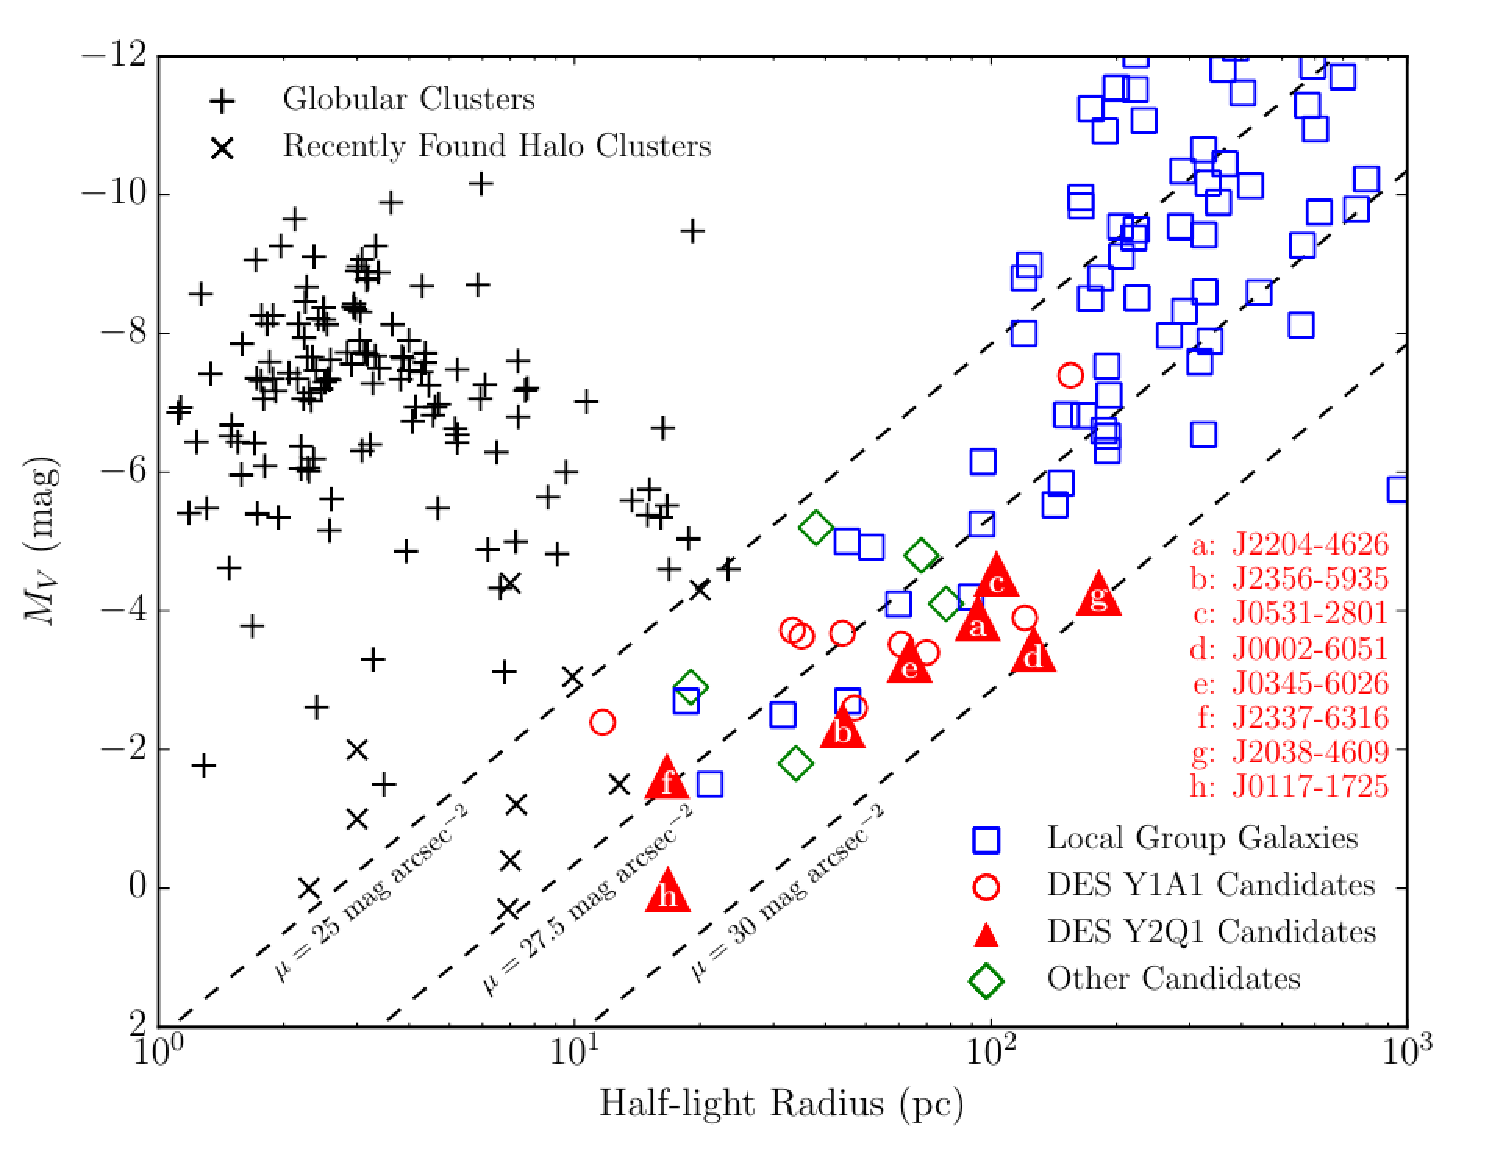
\includegraphics[width=12cm]{figuras/localgroup.pdf}
\caption{\textit{Galáxias do Grupo Local e aglomerados globulares ocupam regiões distintas no plano de raio a meia luz e magnitude absoluta. A maioria dos candidatos a satélite da Galáxia (círculos e triângulos vermelhos) são mais consistentes com o locus de galáxias anãs do Grupo Local (quadrados azuis)  do que com o locus de aglomerados globulares (cruzes pretas). Outras recentes descobertas de candidatos a galáxias anãs estão representadas pelos losangos verdes. Sistemas com identificação ambígua estão marcados pelo x \cite{2013ApJ...767..101B, 2015arXiv150802381L}}}

\label{fig:localgroup}
\end{center}
\end{figure}
\vspace{0.5cm}


Outra descoberta, liderada pelo nosso grupo de pesquisa, foi a detecção do objeto compacto DES 1 \cite{2015arXiv150802381L}. Este objeto é diretamente visto como sobredensidade de fontes azuis nas imagens coadd do DES figura \ref{fig:des1}\footnote{Créditos da imagem \cite{2015arXiv150802381L}}. Na figura \ref{fig:mapdes1}\footnote{Créditos da imagem \cite{2015arXiv150802381L}}, painéis superiores, mostramos a densidade de estrelas em torno do objeto, no painel esquerdo mostramos todas as fontes classificadas como estrelas, como descrito no capítulo \ref{cha:dados},  no painel central mostramos somente as estrelas que estão próximas da isócrona ajustada, veja figura \ref{fig:isodes1}\footnote{Créditos da imagem \cite{2015arXiv150802381L}}. Uma sobredensidade clara e compacta pode ser vista em ambos os painéis. No painel superior direito temos o perfil de significância de Poisson, que mostra um pico de densidade bem pronunciado para cerca de $1'.0$ do centro do objeto. O perfil de significância de Poisson é construído a partir do número de estrelas internas ao raio r e em excesso ao número de estrelas de campo (Nbgd), (Nobj), contra a flutuação esperada no campo. Os painéis inferiores da figura \ref{fig:mapdes1} mostram que não há sobredensidade de galáxias na posição de DES 1. Sendo, portanto, pouco provável que galáxias classificadas erroneamente possam ter contribuído para sobredensidade de DES 1.    

\begin{figure}[h]
\begin{center}
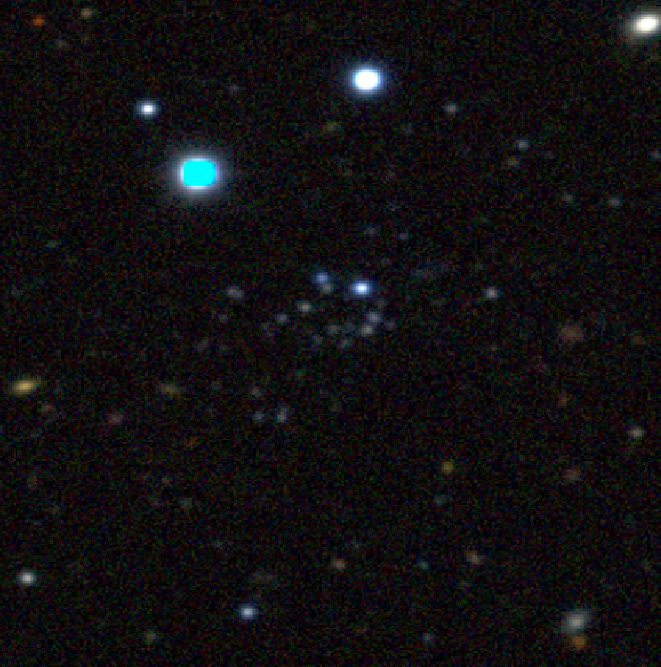
\includegraphics[width=12cm]{figuras/des1.pdf}
\caption{\textit{imagem coadd do DES, cortada em torno de DES 1. Esta imagem foi obtida através do Science portal do DES. A imagem tem  dimensões de $1.'78 × 1.'78  $ e está centrada no objeto  DES 1. A imagem é uma combinação dos filtros g, r e i. }}
\label{fig:des1}
\end{center}
\end{figure}
\vspace{0.5cm}

\begin{figure}[h]
\begin{center}
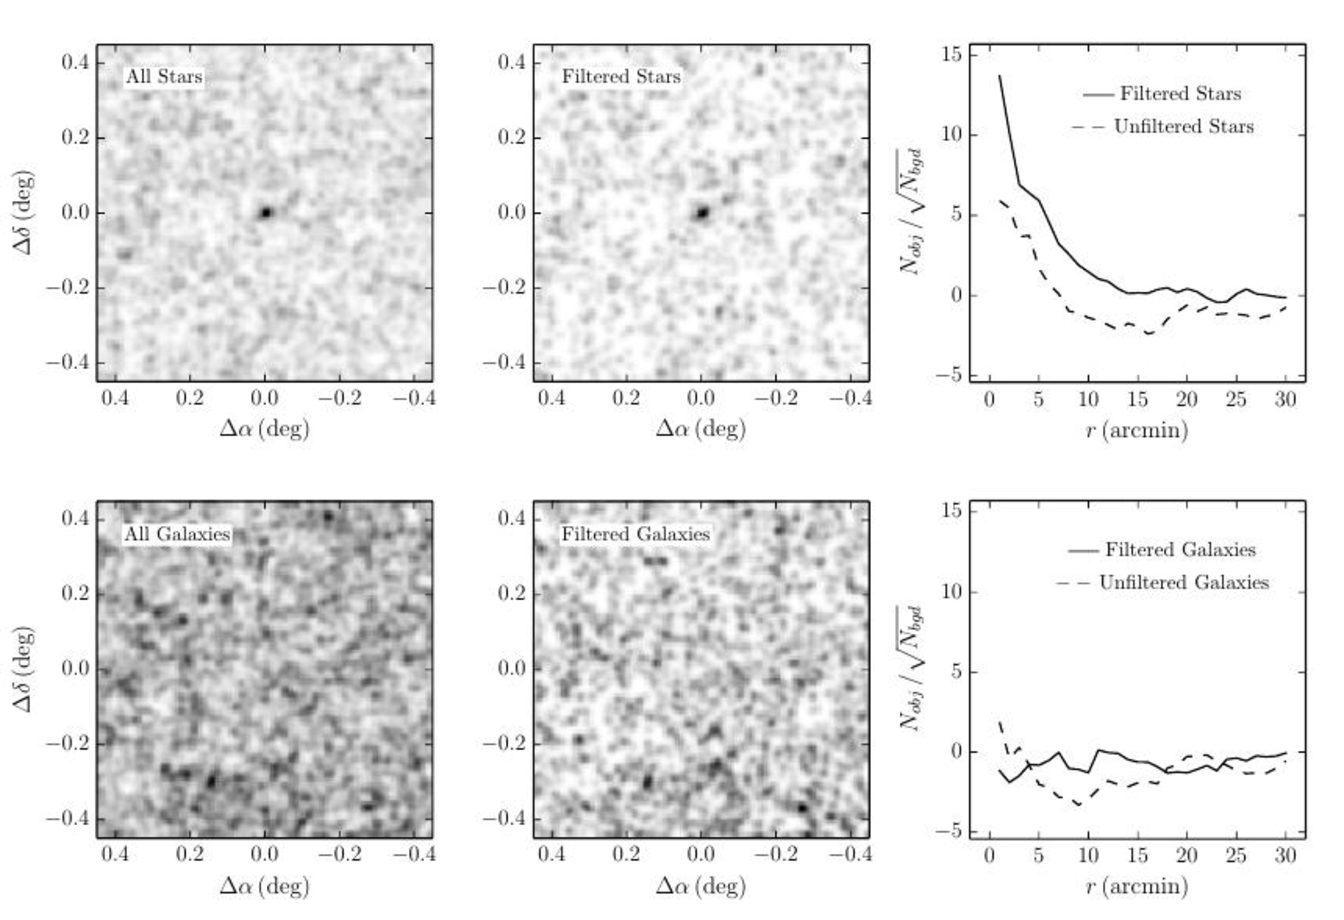
\includegraphics[width=12cm]{figuras/mapdes1.pdf}
\caption{\textit{Painel esquerdo superior: mapa da densidade numérica de fontes estelares em torno de DES 1. Painel superior central: mapa de densidade numéria das estrelas consistentes com o ajuste de isócrona para DES 1 \ref{fig:isodes1}. Painel superior direito: Significância como função radial a partir do centro de DES 1. A linha sólida corresponde a todas as estrelas e a tracejada às estrelas próximas da isócrona ajustada. Os painéis inferiores mostram os mesmos plots usando a distribuição de fontes classificadas como galáxias. Estes mapas foram suavizados com um kernel gaussiano de desvio padrão igual à $0.^{o}03$.}}
\label{fig:mapdes1}
\end{center}
\end{figure}
\vspace{0.5cm}
Mostramos o CMD ajustado para DES 1 no painel esquerdo da figura \ref{fig:isodes1}. Foram plotadas somente estrelas dentro do raio correspondente ao pico do perfil de densidade de Poisson , \ref{fig:mapdes1}. O painel central da figura \ref{fig:isodes1} mostra o CMD para as estrelas de campo. As estrelas deste CMD foram selecionadas como pertencentes a  um anel,  de área igual ao CMD de DES 1 e centrado neste objeto, com um raio interno 10x maior que o raio de DES1. Mostramos também na \ref{fig:isodes1} a melhor isócrona de PADOVA ajustada \cite{2012MNRAS.427..127B}, correspondente a um índice de ferro de $[Fe/H] = −1.88 \pm 0.25$, uma idade de $Log(anos) = 10.00 \pm 0.09$ e módulo de distância de $(m-M) = 19.70 \pm 0.36$. 


\begin{figure}[h]
\begin{center}
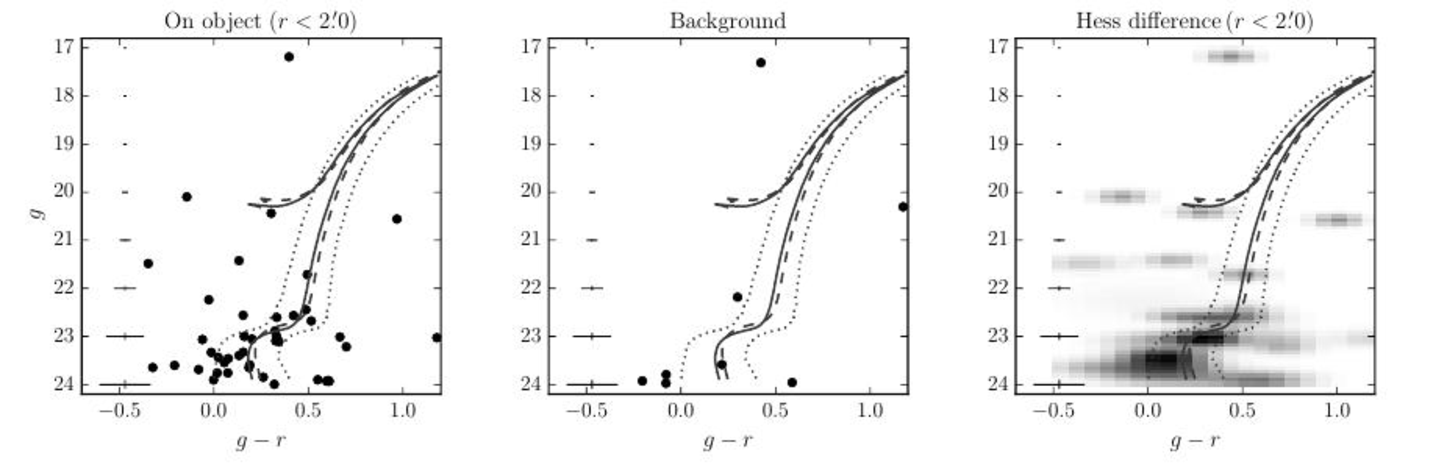
\includegraphics[width=16cm]{figuras/isodes1.pdf}
\caption{\textit{Painel esquerdo CMD das estrelas dentro de $2'.0$ do centro de DES 1. As isócronas com o melhor ajuste exponencial (linha sólida) e o melhor ajuste de perfil de King (linha tracejada) são mostradas, também mostramos linhas pontilhadas definindo os  membros mais prováveis  da população. Painel central: CMD das estrelas de campo, em uma área igual ao painel esquerdo. Painel direito: Diagrama de Hess para a diferença entre os CMDs dos painéis esquerdo e o central.}}
\label{fig:isodes1}
\end{center}
\end{figure}
\vspace{0.5cm}




% ----------------------------------------------------------
% Finaliza a parte no bookmark do PDF
% para que se inicie o bookmark na raiz
% e adiciona espaço de parte no Sumário
% ----------------------------------------------------------
\phantompart

% ---
% Conclusão
% ---
\chapter{Considerações finais}
% ---
Segundo os resultados apresentados no capítulo \ref{cha:validacao} e \ref{cha:dadosdes}, podemos afirmar que o método SparSEx é capaz de encontrar subestruturas da Galáxia como, galáxias anãs, aglomerados globulares e também correntes estelares. Foram recuperadas nos dados do SDSS 11 galáxias anãs \cite{2007ApJ...654..897B,2006AAS...20917805Z}, 4 aglomerados globulares \cite{2007ApJ...669..337K,2002ApJS..141..123W,2010ApJ...712L.103B} e 2 objetos com classificação ambígua \cite{2011MNRAS.416..393B,2010ApJ...712L.103B}. Todos estes objetos foram detectados pelo SparSEx com um ranqueamento alto, ou seja, de todos os candidatos a subestrutura encontrados pelo método, estes foram os mais prováveis. A detecção da corrente estelar da galáxia anã de Sagitário também é bem clara. E traz vantagens em relação aos métodos que usam somente uma SSP, pois geralmente correntes estelares cobrem diferentes distâncias ao longo de sua extensão e algumas apresentam também diferentes metalicidades e idades \cite{2012ApJ...750...80K}. \par
Podemos dizer, portanto, que o SparSEx é um método bem geral na busca de subestruturas, já que ele é capaz de detectar estruturas sem informação prévia da população estelar e também pode detectar objetos com características estruturais bem distintas, como correntes estelares e aglomerados globulares. \par
Também reportamos a descoberta de 17 satélites da Galáxia que foram detectados pelo SparSEx e por outros dois métodos de dentro da colaboração do DES  \cite{2015ApJ...807...50B,2015arXiv150803622T,2015arXiv150802381L}. Essa busca foi feita nos dados correspondentes ao dois primeiros anos do DES, projeto que ainda coletará dados até 2018. A maioria desses objetos tem características consistentes com galáxias anãs, como brilhos superficiais baixos e tamanhos físicos $\ge 40pc$. Um follow-up espectroscópico é necessário para termos certeza sobre a classificação desses objetos. A maioria dos satélites está concentrada perto das nuvens de Magalhães, configuração que pode ter resultado da sua formação concomitante com essas galáxias (satélites de satélites). Além disso, constatamos a existência de um grupo de satélites aglomerados na constelação de Tucana, com cada satélite posicionado a $\le10kpc$ do centróide do grupo. \par
Mostramos também a descoberta do satélite DES 1, que tem uma densidade estelar significativa na sua distribuição espacial e no seu CMD. Os ajustes de isócronas, feitos a partir de dois métodos diferentes, resultaram em uma população velha e pobre em metal, como é de se esperar para estruturas que habitam o halo Galáctico. Ajustes do perfil King usando máxima verossimilhança resultaram em um raio de core de r\textsubscript{c} $\approx 0’.8$ que a uma distância  de 77.6kpc nos leva a um raio físico de  $\approx 9.88 pc$. A magnitude absoluta de DES 1, foi determinada de formar similar a de \cite{2015ApJ...805..130K}, resultando em um valor de $M\textsubscript{v} \approx -3.05$. Esse valor de magnitude absoluta e de tamanho físico para DES 1, o coloca no locus ocupado por aglomerados globulares de baixa luminosidade. DES 1 seria um dos aglomerados globulares mais distantes do Sol, de acordo com a sua distância estimada. \par
Desenvolvemos o SparSEx com o intuito de aplicações em grandes levantamentos de dados como o SDSS e o DES. Mostramos a partir da validação e detecção de objetos, que esse método tem grande potencial para ser aplicado nesses levantamentos. Os próximos anos de observação do DES não irão crescer significativamente em área do céu. Porém, ainda haverá um considerável aumento na profundidade dos dados, o que resulta em um volume efetivo maior coberto. Portanto pretendemos fazer aplicações do SparSEx nas próximas temporadas do DES e também em futuros levantamentos fotométricos como o LSST, descobrindo assim satélites mais fracos, mais distantes  e com brilho superficial mais baixo.


%\lipsum[31-33]

% ----------------------------------------------------------
% ELEMENTOS PÓS-TEXTUAIS
% ----------------------------------------------------------
\postextual
% ----------------------------------------------------------

% ----------------------------------------------------------
% Referências bibliográficas
% ----------------------------------------------------------
\bibliography{bib}
\bibliographystyle{abntex2-alf}

% ----------------------------------------------------------
% Glossário
% ----------------------------------------------------------
%
% Consulte o manual da classe abntex2 para orientações sobre o glossário.
%
%\glossary



%---------------------------------------------------------------------
% INDICE REMISSIVO
%---------------------------------------------------------------------
\phantompart
\printindex
%---------------------------------------------------------------------

\end{document}
